\documentclass[review, 3p, authoryear]{elsarticle} %review=doublespace preprint=single 5p=2 column
%%% Begin My package additions %%%%%%%%%%%%%%%%%%%

\usepackage[hyphens]{url}

  \journal{Journal of Mathematical Psychology} % Sets Journal name

\usepackage{lineno} % add

\usepackage{graphicx}
%%%%%%%%%%%%%%%% end my additions to header

\usepackage[T1]{fontenc}
\usepackage{lmodern}
\usepackage{amssymb,amsmath}
\usepackage{ifxetex,ifluatex}
\usepackage{fixltx2e} % provides \textsubscript
% use upquote if available, for straight quotes in verbatim environments
\IfFileExists{upquote.sty}{\usepackage{upquote}}{}
\ifnum 0\ifxetex 1\fi\ifluatex 1\fi=0 % if pdftex
  \usepackage[utf8]{inputenc}
\else % if luatex or xelatex
  \usepackage{fontspec}
  \ifxetex
    \usepackage{xltxtra,xunicode}
  \fi
  \defaultfontfeatures{Mapping=tex-text,Scale=MatchLowercase}
  \newcommand{\euro}{€}
\fi
% use microtype if available
\IfFileExists{microtype.sty}{\usepackage{microtype}}{}
\usepackage[]{natbib}
\bibliographystyle{plainnat}

\ifxetex
  \usepackage[setpagesize=false, % page size defined by xetex
              unicode=false, % unicode breaks when used with xetex
              xetex]{hyperref}
\else
  \usepackage[unicode=true]{hyperref}
\fi
\hypersetup{breaklinks=true,
            bookmarks=true,
            pdfauthor={},
            pdftitle={Combining support for hypotheses over heterogeneous studies with Bayesian Evidence Synthesis: A simulation study},
            colorlinks=false,
            urlcolor=blue,
            linkcolor=magenta,
            pdfborder={0 0 0}}

\setcounter{secnumdepth}{5}
% Pandoc toggle for numbering sections (defaults to be off)


% tightlist command for lists without linebreak
\providecommand{\tightlist}{%
  \setlength{\itemsep}{0pt}\setlength{\parskip}{0pt}}

% From pandoc table feature
\usepackage{longtable,booktabs,array}
\usepackage{calc} % for calculating minipage widths
% Correct order of tables after \paragraph or \subparagraph
\usepackage{etoolbox}
\makeatletter
\patchcmd\longtable{\par}{\if@noskipsec\mbox{}\fi\par}{}{}
\makeatother
% Allow footnotes in longtable head/foot
\IfFileExists{footnotehyper.sty}{\usepackage{footnotehyper}}{\usepackage{footnote}}
\makesavenoteenv{longtable}



\usepackage{booktabs}
\usepackage[section]{placeins}
\usepackage{float}
\usepackage{caption}
\captionsetup[figure]{font=footnotesize,skip=3pt}



\begin{document}


\thispagestyle{empty}

\begin{large}
\noindent Research Master's programme 
Methodology and Statistics for the Behavioural, Biomedical and Social Sciences \newline
Utrecht University, the Netherlands \newline
\newline
\newline
\newline
\newline
MSc Thesis Thom Volker (5868777) 
\newline
TITLE: "Combining support for hypotheses over heterogeneous studies with Bayesian Evidence Synthesis: A simulation study" 
\newline
May 2022 
\newline
\newline
\newline
\newline
\newline
Supervisor:\newline
Prof. Dr. Irene Klugkist \newline
\newline
\newline
Second grader: \newline
Prof. Dr. Ir. Bernard Veldkamp
\newline
\newline
\newline
\newline
Preferred journal of publication: Journal of Mathematical Psychology 
\newline
Word count: 9839
\newline
\end{large}
\addtocounter{page}{-1}
\clearpage
\pagebreak


\begin{frontmatter}

  \title{Combining support for hypotheses over heterogeneous studies with Bayesian Evidence Synthesis: A simulation study}
    \author[Utrecht University]{Thom Benjamin Volker%
  \corref{cor1}%
  \fnref{1}}
   \ead{t.b.volker@uu.nl} 
      \affiliation[Utrecht University]{Department of Methodology and Statistics, Padualaan 14, Utrecht}
    \cortext[cor1]{Corresponding author}
    \fntext[1]{I gratefully acknowledge stimulating discussions with Prof.~Dr.~Ir. Vincent Buskens and Prof.~Dr.~Werner Raub.}
  
  \begin{abstract}
  Scientific claims gain credibility by replicability, especially if replication under different circumstances and varying designs yields equivalent results. Aggregating results over multiple studies is, however, not straightforward, and when the heterogeneity between studies increases, conventional methods as (Bayesian) meta-analysis and Bayesian sequential updating become infeasible. \emph{Bayesian Evidence Synthesis}, built upon the foundations of the Bayes factor, allows to aggregate the support for conceptually similar hypotheses over studies, regardless of methodological differences. We assess the performance of Bayesian Evidence Synthesis over multiple effect and sample sizes, with a broad set of (inequality-constrained) hypotheses using Monte Carlo simulations, focusing explicitly on the complexity of the hypotheses under consideration. The simulations show that this method can evaluate complex (informative) hypotheses regardless of methodological differences between studies, and performs adequately if the set of studies considered has sufficient statistical power. Additionally, we pinpoint challenging conditions that can lead to unsatisfactory results, and provide suggestions on how to handle these situations.
  \end{abstract}
    \begin{keyword}
    Bayes factors \sep replication \sep hypothesis evaluation \sep informative hypotheses \sep 
    research synthesis
  \end{keyword}
  
 \end{frontmatter}

\widowpenalty10000
\clubpenalty10000

\hypertarget{introduction}{%
\section{Introduction}\label{introduction}}

In recent years, a meta-analytic way of thinking has been advocated in the scientific community.
This approach is grounded in the belief that a single study is merely contributing to a larger body of evidence \citep[e.g.,][]{asendorpf_recommendations_2016, cumming_new_2014, goodman_reproducibility_2016}.
Such evidence gains credibility only by replicability of the findings with new data \citep{schmidt_replication_2009}, because the ability to replicate research findings ensures that the findings represent \emph{true} phenomena rather than artefacts.
The replication crisis in the social sciences placed the importance of replication back on the research agenda and kickstarted multiple replication initiatives.
Accordingly, multiple efforts aimed at fostering replication were undertaken, such as journals or journal sections devoted to replication studies (e.g., Royal Society Open Science, Registered Replication Reports, Journal of Personality and Social Psychology) and grant opportunities for replication studies \citep[e.g.,][]{nwo_replication_2020}.
Moreover, multiple scholars legitimately emphasized the importance of replication studies for the future of science \citep[e.g.,][]{baker_reproducibility_2016, brandt_et_al_replication_2014, munafo_manifesto_2017}.

This renewed interest in replication was mostly directed toward studies that are highly similar, using a methodology and research design that mimics the original study as closely as possible \citep[e.g.,][]{camerer2016evaluating, camerer2018evaluating, klein_etal_replicability_2014, nosek_replicability_review_2021, open_science_collab_2015}.
These studies, commonly referred to as \emph{direct}, \emph{exact} or \emph{close} replications, are primarily concerned with the statistical reliability of the results.
As such, direct replications are tailored towards assessing whether or not the results of the initial study are due to chance.
Agreement between the findings of a direct replication and the findings of the initial study increases the confidence in the accuracy of the original findings.
However, direct replicability is a necessary but insufficient condition for making scientific claims.
If the results of the studies depend on methodological flaws, inferences from all studies will lead to suboptimal or invalid conclusions \citep{lawlor_triangulation_2017, munafo_robust_2018}.

\emph{Conceptual} replications protect against placing too much confidence in findings that depend on methodological shortcomings.
A conceptual replication primarily assesses the validity and generalizability of a study, by testing whether similar results can be obtained under different circumstances, or using different methods and operationalizations \citep{nosek_scientific_2012}.
The idea is that a phenomenon that can be observed in a variety of research settings is more likely to represent a \emph{true} effect than a finding that replicates only in particular circumstances \citep{crandall_conceptual_2016}.
Additionally, different methodologies used in different studies may have different strengths and weaknesses, that may all affect the conclusions drawn from the data.
Combining evidence from multiple approaches mitigates the effect of these strengths and weaknesses, and thereby enhances the validity and the robustness of the final conclusion \citep{lawlor_triangulation_2017, lipton2003inference, mathison1988triangulate, munafo_robust_2018, nosek_scientific_2012}.

In the conventional framework of direct replications, combining evidence over studies is relatively straightforward, because established methods as (Bayesian) meta-analysis or Bayesian sequential updating can be applied to aggregate the results \citep{lipsey_wilson_2001, schonbrodt_sequential_2017, sutton_bayesian_meta2001}.
These methods pool the parameter estimates or effect sizes obtained in the individual studies \citep{cooper_handbook_2009}.
Even if the studies are not identical, but still considerably similar in terms of study design and analysis methods, meta-analysis can be used, and moderators can be added to explain variability in the estimated effects.
However, if the studies differ considerably with regard to research design, operationalizations of key variables or statistical models used, the parameter estimates or effect sizes will not be comparable.
Consequently, an aggregate of these estimates cannot be meaningfully interpreted, which renders the use of such conventional approaches unfeasible.
This problem complicates the quantification of the evidence for a scientific claim over multiple studies that, although conceptually similar, differ methodologically.

To overcome this problem, \citet{kuiper_combining_2013} proposed a new method called \emph{Bayesian Evidence Synthesis} (\emph{BES}).
At its core, \emph{BES} quantifies the support for a scientific theory or an overarching hypothesis by aggregating Bayes factors obtained in individual studies.
In every single study, a statistical hypothesis can be formulated that reflects the overall theory, but that incorporates data characteristics and research methodology unique to that study.
The support for each study-specific hypothesis can be expressed using a Bayes factor (\(BF\)), rendering the relative support for the hypothesis of interest over an alternative hypothesis \citep{kass_raftery_bayes_factors_1995}.
If the study-specific hypotheses represent the same underlying (i.e., latent) effect, the Bayes factors on these hypotheses can be meaningfully combined.
After all, each individual study provides a certain amount of evidence for or against the overarching theory.
The evidence in each study can be aggregated into a single measure that reflects the support for the theory over all studies combined.

In the context of individual studies, the popularity of Bayesian statistics in general \citep[e.g.,][]{lynch_bayesian_2019} and Bayesian hypothesis evaluation specifically \citep{vandeschoot_systematic_2017}, rapidly increased over recent years.
In contrast to the classical null hypothesis testing paradigm, the Bayesian hypothesis evaluation enables researchers to compare a wide range of potentially non-nested hypotheses that may have multiple equality- and order-constraints, by balancing the fit of the hypotheses to the data with the complexity of the candidate hypotheses \citep{klugkist_inequality_2005, hoijtink2019tutorial}.
Additionally, the Bayesian framework allows to quantify the amount of evidence from the data for or against the hypothesis of interest, rather than merely assessing whether the classical null hypothesis can be rejected \citep{Wagenmakers_bayesian_2018}.
As such, Bayesian hypothesis evaluation provides a flexible framework that can be applied to a broad range of scientific hypotheses, which allows to quantify the evidence for or against hypotheses over a diverse set of studies.
Yet, although the theoretical foundations of \emph{BES} have been laid out by \citet{kuiper_combining_2013}, and the method has been applied successfully in substantive research \citep[e.g.,][]{kevenaar_bes_2021, zondervan_parental_2019, zondervan_robust_2020, volker_cooperation_2022}, empirical research on Bayesian evaluation of hypotheses has hardly been extended to the case in which evidence is combined over multiple studies.
It is not obvious how research on Bayes hypothesis evaluation within studies translates to the situation in which evidence is combined over multiple studies.
As a consequence, the necessary conditions for adequate performance of \emph{BES} should receive further scrutiny.

In this paper, we assess the performance of \emph{BES} in various scenarios relevant to applied researchers.
In multiple simulations, we apply \emph{BES} to aggregate the evidence for conceptually similar hypotheses that are evaluated using different statistical models, while varying the operationalizations of key variables concerned by the hypothesis.
We restrict the simulations to the evaluation of regression coefficients in three members of the generalized linear model family: ordinary least squares (OLS), logistic and probit regression, because of their widespread appearance in empirical research.
Note, however, that the applicability of \emph{BES} reaches beyond these methods: as long as a conceptually similar hypothesis on the parameters of the models can be evaluated using Bayes factors, \emph{BES} can be used to aggregate the results.
Yet, exactly this flexibility may pose challenges to the application of \emph{BES}.
Different operationalizations of key variables affect the complexities of the hypotheses evaluated in the individual studies.
Consequently, the Bayes factors within these studies are affected by the complexities of the hypotheses, such that the resulting amount of evidence may largely depend on the specification of the hypothesis, rather than on the veracity of the hypotheses.
Our simulations assess how common procedures in data handling affect the complexities of the hypotheses and the resulting performance of \emph{BES}.
Additionally, we investigate in which situations \emph{BES} does not perform adequately, and provide suggestions on how such situations can be handled.
Yet, before discussing turning to the simulations, a detailed description of \emph{BES} tailored to the specification of the simulation study is provided.
The paper concludes with an extensive discussion of the implications of the simulations.

\hypertarget{aggregating-evidence-with-bes}{%
\section{\texorpdfstring{Aggregating Evidence with \emph{BES}}{Aggregating Evidence with BES}}\label{aggregating-evidence-with-bes}}

Using \emph{BES} to quantify the evidence for a scientific theory requires three building blocks.
First, \emph{BES} requires multiple studies on the same phenomenon, that all assess a conceptually similar hypothesis \citep{kuiper_combining_2013}.
Hence, in each study, a hypothesis must be formulated that reflects this scientific theory, but that also accounts for the specifics of the study, such as the empirical design, the analysis model and operationalizations of key variables.
Second, these hypotheses are evaluated in each study separately.
In the Bayesian framework, this is done by estimating the posterior distribution of the parameters of the model, after which the fit of the model to the hypothesis is quantified using a Bayes factor.
Third, the support for the theory in each individual study is aggregated using an updating procedure, that renders the support for the theory over all studies combined.
Each of these steps are outlined in more detail in the current section.

\hypertarget{informative-hypotheses}{%
\subsection{Informative hypotheses}\label{informative-hypotheses}}

When translating a conceptual hypothesis (i.e., the scientific theory) to a statistical hypothesis, researchers conventionally relied on the null hypothesis testing framework.
In the context of regression models, this generally implies that researchers evaluate the null hypothesis, \(H_0\), stating that the regression coefficients \(\beta_k\) (where \(k\) is an indicator) equal zero, against an unconstrained alternative hypothesis, \(H_u\), indicating that they can have any value.
Several authors emphasized shortcomings of this approach, remarking that the ability to reject a null hypothesis is hardly illuminating, because the null is seldom (exactly) true \citep{cohen_earth_1994, lykken_wrong_1991} and rarely corresponds to the expectations researchers have \citep{cohen_things_i_learned_1990, vandeschoot_informative_2011, royall1997statistical, trafimow_manipulating_2018}.
Multiple researchers argued that scientific expectations can be better captured in an informative hypothesis \citep{hoijtink_informative_2012, vandeschoot_informative_2011}.

Informative hypotheses allow to formalize the expectations researchers have on the parameters of the statistical model \citep{hoijtink_informative_2012}.
Rather than expecting that the regression coefficients under evaluation are equal to zero, researchers may, for instance, expect that all are positive.
In a regression model with three predictors, this expectation yields
\[
H_i: \{\beta_1, \beta_2, \beta_3\} > 0.
\]
However, informative hypotheses are not restricted to inequality-constrained hypotheses.
An informative hypothesis might contain equality and inequality constraints between parameters and between combinations of parameters, as well as expectations regarding effect sizes or range constraints \citep{hoijtink2019tutorial}.
Combining these features allows great flexibility to researchers to formalize their theories, potentially resulting in fairly complex hypotheses.
For example, the expectation that \(\beta_1\) and \(\beta_2\) are of the same size, while both are positive but smaller than \(\beta_3\), can be formalized as
\[
H_{i'}: 0 < \{\beta_1=\beta_2\} < \beta_3. 
\]
The flexibility with regard to specifying hypotheses is especially advantageous in the context of \emph{BES}, where studies may differ in the operationalizations of key variables, and thus in the hypotheses that are evaluated.

\hypertarget{hypothesis-evaluation-using-the-bayes-factor}{%
\subsection{Hypothesis evaluation using the Bayes factor}\label{hypothesis-evaluation-using-the-bayes-factor}}

Within the Bayesian framework, the support for (informative) hypotheses can be expressed in terms of a Bayes factor \citep{kass_raftery_bayes_factors_1995}.
Bayes factors require that a likelihood function (i.e., an analysis model for the data) is combined with a prior distribution, resulting in the posterior distribution of the parameters.
The posterior distribution can subsequently be used to calculate the Bayes factor, which quantifies the relative support for a hypothesis over some alternative.

\hypertarget{likelihood-of-the-parameters}{%
\subsubsection{Likelihood of the parameters}\label{likelihood-of-the-parameters}}

After formulating the hypotheses of interest, researchers need to specify a statistical model (i.e., a likelihood function) that is compatible with these hypotheses and that can be used to analyse the data \citep{lynch_introduction_2007}.
A likelihood function quantifies the support in the data for each potential parameter value.
This paper solely focuses on OLS, logistic and probit regression, which are all part of the generalized linear model (GLM) family (note that there are many other models that fall under the GLM family).
GLMs extend the linear regression model to deal with response variables that are assumed to follow an exponential distribution, by using a link function \(g(\boldsymbol{\mu}) = X\beta\), with \(X\) an \(n \times p\) matrix containing \(n\) observations' scores on \(p\) predictor variables, \(\beta\) is a \(p \times 1\) vector containing the regression coefficients, and \(\boldsymbol{\mu} = E(Y|X)\), where \(Y\) is an \(n \times 1\) vector with response values.
The purpose of the link function is to model each observation's expected response \(E(Y|X)\) in terms of a linear combination of the predictor variables.
Accordingly, the likelihood of the parameters given the data under the generalized linear model is formalized as
\[
L(\beta, \phi|Y, X) \equiv f(Y|X, \beta, \phi) = \prod^n_{i=1} f(Y_i|X_i \beta, \phi),
\]
where \(i\) is an indicator for each individual observation and \(\phi\) denotes the variance or dispersion parameter.

One of the best known models in the class of GLMs is the linear regression model, which uses the identity link function, such that \(g(\boldsymbol{\mu}) = \boldsymbol{\mu} = X\beta\).
The likelihood function of the linear regression model is defined by
\[
f(Y | X, \beta, \phi) = \prod^n_{i=1} \frac{1}{\sqrt{2\pi\sigma^2}} \text{exp}
\Bigg\{
- \frac{(Y_i - X_i\beta)^2}{2\sigma^2}
\Bigg\},
\]
where \(\phi = \sigma^2\).
When the outcome \(Y\) to be modeled is dichotomous rather than continuous, the binomial distribution can be used.
The corresponding likelihood is defined by
\[
f(Y|X, \beta) = \prod^n_{i=1} p_i^{Y_i} (1 - p_i)^{1 - Y_i},
\]
where \(Y_i\) is either \(0\) or \(1\), and \(p_i\) is specified according to the logit link \(g(\boldsymbol{\mu}) = \text{ln}\Big(\frac{\boldsymbol{\mu}}{1 - \boldsymbol{\mu}}\Big) = X\beta\) for logistic regression, or probit link \(g(\boldsymbol{\mu}) = \Phi^{-1}(\boldsymbol{\mu}) = X\beta\), where \(\Phi^{-1}\) is the inverse cumulative standard normal distribution, for probit regression models.
The dispersion parameter is omitted because it equals \(\phi = 1\) for logistic and probit models.

\hypertarget{prior-distribution}{%
\subsubsection{Prior distribution}\label{prior-distribution}}

After specifying the analysis model, the prior distribution for the model parameters must be defined.
Because the prior for an informative hypothesis can be obtained by truncating the unconstrained (or encompassing) prior \citep[e.g.,][]{klugkist_inequality_2005}, we first discuss the latter.
The prior distribution reflects which parameter values are most likely before observing the data, and hence may be more or less informative depending on the amount of prior knowledge researchers have.
Although researchers have substantial freedom in specifying the prior distribution, inadequate choices have adverse consequences for hypothesis evaluation and comparison, rendering it a complicated task \citep{ohagan_fractional_1995}.
A practical solution to the specification of the prior for hypothesis evaluation, is to use a fractional unconstrained prior \citep{ohagan_fractional_1995} that protects against a subjective specification \citep{gu_approximated_2018}.
This approach entails that a non-informative improper prior is updated with a small fraction \(b = \frac{J}{n}\) of the information in the data (i.e., the likelihood), resulting in a proper default prior distribution \citep[e.g.,][]{mulder_equality_2010, gu_approximated_2018}, such that
\[
p_u(\beta, \phi|Y, X, b) = 
\frac{
  p_u(\beta, \phi) ~ f(Y|X, \beta, \phi)_b
}{
  \int \int p_u(\beta, \phi) ~ f(Y|X, \beta, \phi)_b ~ \partial \beta \partial \phi
}.
\]
\citet{mulder_olssoncollentine_2019} proved that, under the linear model, updating a noninformative improper Jeffrey's prior with a fraction \(b = \frac{p+1}{n}\) of the likelihood renders a Student \(\mathcal{T}\) prior distribution with 1 degree of freedom (i.e., a Cauchy distribution) for the regression coefficients,
\[
p_u(\beta | Y, X, b) = \mathcal{T}(\hat{\beta}, \hat{\Sigma}_\beta / b, 1),
\]
with location parameter \(\hat{\beta}\) (the maximum likelihood estimates of the regression coefficients) and scale parameter \(\Sigma_{\beta} / b\) (the covariance matrix of the regression coefficients over \(b\)). A discussion of a prior for the dispersion parameter is omitted, because nuisance parameters are integrated out when calculating Bayes factors \citep[e.g.,][]{gu_approximated_2018}.

When the model under evaluation is not (multivariate) normal, but another GLM, obtaining an analytically tractable posterior may be more difficult, regardless of the choice of prior \citep{bda2013}.
Nevertheless, large-sample theory dictates that a fractional prior for the regression coefficients can be approximated by a multivariate normal distribution \citep{bda2013}.
In this case, \citet{gu_approximated_2018} showed how a fractional prior can be obtained by updating a non-informative prior with a fraction \(b = \frac{J}{n}\) of the likelihood.
This approach renders an approximately normal prior distribution for the regression coefficients
\[
p_u(\beta | Y, X, b) \approx \mathcal{N}(\hat{\beta}, \Sigma_\beta / b).
\]
with mean vector \(\hat{\beta}\) and covariance matrix \(\Sigma_{\beta}/b\) (the unbiased estimate of the covariance matrix of the regression coefficients over the fraction \(b\)).
Under this approach \(J\) typically equals the number of independent constraints in all hypotheses of interest within a study, although different specifications are possible \citep[for an elaborate discussion on appropriate values for \(J\), see][]{gu_approximated_2018, hoijtink_prior_2021}.

After specifying a prior for the unconstrained hypothesis, the encompassing prior approach can be used to obtain a prior for an informative hypothesis by truncating the unconstrained prior \citep[e.g.,][]{klugkist_inequality_2005, mulder_equality_2010, mulder_prior_2014}.
Accordingly, the prior for an informative hypothesis is proportional to the region of the prior that is in agreement with the constraints imposed by the hypothesis under consideration.
That is, \(p_i(\beta | Y, X, b) \propto p_u(\beta | Y, X, b)\boldsymbol{1}_{\boldsymbol{B_i}}\), where \(\boldsymbol{1}_{\boldsymbol{B_i}}\) is an indicator for the parameter space that is in line with hypothesis \(H_i\) \citep{gu_approximated_2018}.

\hypertarget{posterior-distribution}{%
\subsubsection{Posterior distribution}\label{posterior-distribution}}

Combining the likelihood of the parameters with the prior distribution yields the posterior distribution.
The posterior quantifies the support and for each parameter value after observing the data.
Under the fractional prior approach, the unconstrained fractional prior is updated with the remaining fraction \(1-b\) of the likelihood.
This approach yields the posterior distribution under an unconstrained hypothesis
\[
P_u(\beta, \phi | Y, X) = 
\frac{
f(Y | X, \beta, \phi)_{1-b} ~ p_u(\beta, \phi | Y, X, b)
}{
\int \int f(Y | X, \beta, \phi)_{1-b} ~ p_u(\beta, \phi | Y, X, b) ~ \partial \beta ~ \partial \phi
},
\]
where \(f(Y | X, \beta, \phi)_{1-b}\) yields the fraction \(1-b\) of the likelihood.
\citet{mulder_olssoncollentine_2019} proved that updating a \(\mathcal{T}(B_0, \Sigma_b, 1)\) prior distribution with the remaining fraction of the likelihood of the normal linear model yields a multivariate Student \(\mathcal{T}\) posterior distribution
\[
P_u(\beta | Y, X) = \mathcal{T}(\hat{\beta}, \Sigma_\beta, n - k),
\]
with location parameter \(\hat{\beta}\), scale parameter \(\Sigma_{\beta}\) and \(df = n - k\) degrees of freedom.\footnote{Similarly to the prior distribution, nuisance parameters are integrated out when calculating the Bayes factor, and therefore a discussion of the posterior distribution is omitted for these parameters.}

For GLMs other than the linear model, as well as hierarchical and structural equation models, \citet{gu_approximated_2018} discussed how the posterior distribution of the regression coefficients can be approximated by a multivariate normal distribution, which yields
\[
P_u(\beta | Y, X) \approx \mathcal{N}(\hat{\beta}, \Sigma_\beta),
\]
with a posterior mean vector \(\hat{\beta}\), and a posterior covariance matrix \(\Sigma_\beta\).
Because a truncated prior distribution under an informative hypothesis yields a density that is equal to zero at the truncated part of the distribution, and the likelihood function is unaffected by the hypothesis, the posterior distribution under an informative hypothesis also yields a truncated version of the unconstrained posterior.
That is, the posterior distribution under hypothesis \(H_i\) yields
\(P_i(\beta | Y, X) \propto P_i(\beta | Y, X)\boldsymbol{1}_{\boldsymbol{B_i}}\), where \(\boldsymbol{1}_{\boldsymbol{B_i}}\) indicates the region of the parameter space in line with hypothesis \(H_i\).

\hypertarget{bayes-factors}{%
\subsubsection{Bayes factors}\label{bayes-factors}}

The Bayes factor comparing hypotheses \(H_i\) and \(H_{i'}\) is defined as the ratio of the marginal likelihoods of these hypotheses, i.e.,
\[
BF_{ii'} = \frac{m(Y | X, H_i)}{m(Y | X, H_{i'})}.
\]
This measure can be directly interpreted as the evidence in the data for hypothesis \(H_i\) versus the evidence in the data for hypothesis \(H_{i'}\).
As such, if \(BF_{ii'} = 7\), hypothesis \(H_i\) obtains 7 times more support than hypothesis \(H_{i'}\).
The marginal likelihood of hypothesis \(H_i\) is defined as
\[
\begin{aligned}
m(Y | X, H_i) 
&= \int \int_{\beta \in \boldsymbol{B_i}}  P_i(\beta, \phi | Y, X) ~ \partial \beta ~ \partial \phi \\
&= \int \int_{\beta \in \boldsymbol{B_i}} f(Y | X, \beta, \phi) ~ p_i(\beta, \phi | Y, X) ~ \partial \beta ~ \partial \phi,
\end{aligned}
\]
which, when using the fractional prior and posterior, yields
\[
m(Y | X, H_i) = 
  \int \int_{\beta \in \boldsymbol{B_i}}  f(Y | X, \beta, \phi)_{1-b} ~ p_i(\beta, \phi | Y, X, b) ~ \partial \beta ~ \partial \phi.
\]
Whereas, in general, obtaining the marginal distribution is a complicated endeavor, the encompassing prior approach greatly simplifies this task \citep{klugkist_inequality_2005}.
In fact, \citet{gu_approximated_2018} showed that when comparing an informative hypothesis \(H_i\) with an unconstrained hypothesis \(H_u\), the ratio of the two marginal likelihoods boils down to
\[
\begin{aligned}
BF_{iu} &= 
\frac{
  \int \int_{\beta \in \boldsymbol{B_i}} f (Y | X, \beta, \phi)_{1-b} ~ p_i(\beta, \phi | Y, X, b) \partial \beta ~ \partial \phi
}{
  \int \int f(Y | X, \beta, \phi)_{1-b} ~ p_u(\beta, \phi | Y, X, b) \partial \beta ~ \partial \phi
} \\
&= \int \int_{\beta \in \boldsymbol{B_i}} 
\frac{
  f (Y | X, \beta, \phi)_{1-b} ~  \frac{p_u (\beta, \phi | Y, X, b)}{\int \int_{\beta \in \boldsymbol{B_i}} p_u (\beta | Y, X, b) \partial \beta ~ \partial \phi}
}{
  \int \int f(Y|X, \beta, \phi)_{1-b} ~ p_u(\beta | Y, X, b) \partial \beta ~ \partial \phi
} \partial \beta ~ \partial \phi \\
&= \frac{
   \int \int_{\beta \in \boldsymbol{B_i}} P_u(\beta|Y, X) ~ \partial \beta ~ \partial \phi
}{
  \int\int_{\beta \in \boldsymbol{B_i}} p_u(\beta | Y, X, b) \partial \beta ~ \partial \phi
}.
\end{aligned}
\]
That is, the constrained prior can be factored into an unconstrained prior and the marginal constrained prior distribution.
This yields a marginal prior and marginal posterior distribution, evaluated over the parameter space in line with the hypothesis.

In the current definition of the Bayes factor, however, the prior distribution is centered at the maximum likelihood estimates of the regression coefficients, as implied by the fraction of information from the likelihood.
This is problematic when testing inequality-constrained hypotheses (e.g., \(H_i: \beta > 0\) versus \(H_{i'}: \beta \leq 0\)), because one of the two hypotheses obtains a larger prior plausibility unless the estimated coefficient is exactly equal to the boundary of the hypotheses (e.g., \(\hat{\beta}=0\)).
When using a symmetric prior, balancing the unconstrained prior on the boundary of the hypotheses ensures that both hypotheses receive the same \emph{a priori} support.
Additionally, when testing equality-constrained hypotheses, \citet{jeffreys_1961} remarked that centering the prior around the hypothesized value is substantively desirable, because the \emph{a priori} expectation is that the estimate should be close to the hypothesized value, otherwise there is little merit in testing precisely this hypothesis.
Based on these considerations, several scholars advocated to center the prior distribution around the focal point of interest when calculating the Bayes factor \citep{gu_approximated_2018, mulder_prior_2014, zellner_siow_1980, mulder_gu_bayesian_2021}.
This procedure renders the \emph{adjusted} fractional Bayes factor, which is defined by
\[
BF_{iu} = \frac{
  \int \int_{\beta \in \boldsymbol{B}_i} P_u(\beta, \phi | Y, X) ~ \partial \beta ~ \partial \phi
} {
  \int \int_{\beta \in \boldsymbol{B}_i} p^*_u(\beta, \phi| Y, X, b) ~ \partial \beta ~ \partial \phi
},
\]
where the prior for the coefficients is centered around the hypothesized values.
After integrating out the nuisance parameters, this yields
\[
BF_{iu} = \frac{
  \int_{\beta \in \boldsymbol{B_i}} P_u (\beta | Y, X) ~ \partial \beta
}{
  \int_{\beta \in \boldsymbol{B_i}} p^*_u(\beta | Y, X, b) ~ \partial \beta
}
= \frac{f_i}{c_i}.
\]
Consequently, \(BF_{iu}\) is defined as the proportion of the posterior distribution that is in line with hypothesis \(H_i\), denoted fit (\(f_i\)), over the proportion of the adjusted unconstrained prior distribution that is in line with hypothesis \(H_i\), denoted complexity (\(c_i\)).
As such, the Bayes factor serves as Occam's razor, by balancing the fit of the data to the hypothesis (i.e., the marginal posterior) with the complexity of the hypothesis.

This formulation of the Bayes factor is relatively easy to compute for both equality and inequality constrained informative hypotheses.
Namely, when the hypothesis of interest only contains equality constraints, one can make use of the Savage-Dickey density ratio \citep{savage_dickey_1971}, which yields
\[
BF_{i_0u} = \frac{f_{i_0}}{c_{i_0}} = \frac{
  P_u(\beta = \boldsymbol{B_{i_0}} | Y, X)
}{
  p_u^*(\beta = \boldsymbol{B_{i_0}} | Y, X, b)
},
\]
which is the ratio of the densities of the posterior \(P_u(\beta = \boldsymbol{B_{i_0}} | Y, X)\) and adjusted prior \(p^*_u(\beta = \boldsymbol{B_{i_0}} | Y, X, b)\), evaluated at the location of the hypothesized values.
When the hypothesis of interest contains merely inequality constraints, the Bayes factor is expressed as the ratio between the volume of the posterior that is in line with the hypothesis and the volume of the prior that is in line with the hypothesis, such that
\[
BF_{i_1u} = \frac{f_{i_1}}{c_{i1}} = 
\frac{
  \int_{\beta \in \boldsymbol{B_{i_1}}} P_u(\beta | Y, X)
}{
  \int_{\beta \in \boldsymbol{B_{i_1}}} p_u^*(\beta | Y, X, b)
}.
\]
In the most complex scenario where the hypothesis of interest contains both equality and inequality constraints, the Bayes factor equals
\[
BF_{i_{01}u} = \frac{f_{i_{01}}}{c_{i_{01}}} = \frac{
  P_u(\beta_{i_0} = \boldsymbol{B_{i_0}} | Y, X)
}{
  p^*_u(\beta^*_{i_0} = \boldsymbol{B_{i_0}} | Y, X, b)
} \times
\frac{
  \int_{\beta_{i_1} \in \boldsymbol{B_{i_1}}} P_u(\beta_{i_1} | \beta_{i_0} = \boldsymbol{B_{i_0}}, Y, X)
}{
  \int_{\beta_{i_1} \in \boldsymbol{B_{i_1}}} p^*_u(\beta_{i_1} | \beta_{i_0} = \boldsymbol{B_{i_0}}Y, X, b)
},
\]
where \(\beta_{i_0}\) and \(\beta_{i_1}\) are the equality and inequality constrained parameters under the hypothesis, respectively \citep{gu_approximated_2018}.
Additionally, the Bayes factor between two informative hypotheses is easy to calculate due to transitivity of the Bayes factor.
That is, both informative hypotheses can be expressed with reference to the unconstrained hypothesis, such that comparing two informative hypotheses \(H_i\) and \(H_{i'}\) yields
\[
BF_{ii'} = \frac{BF_{iu}}{BF_{i'u}} = \frac{f_i / c_i}{f_{i'}/c_{i'}}.
\]
A special case of an alternative informative hypothesis is a complement hypothesis.
The complement of hypothesis \(H_i\) reads ``not \(H_i\)'' and reflects all possible parameter values outside the constraints imposed by the hypothesis under consideration.
Evaluating a single informative hypothesis against its complement yields
\[
BF_{i, c} = \frac{BF_{i,u}}{BF_{c,u}} = \frac{f_i/c_i}{(1 - f_i) / (1 - c_i)}.
\]
Because a hypothesis and its complement cover mutually exclusive regions of the entire parameter space, evaluating against the complement is more powerful than evaluating against an unconstrained hypothesis \citep{klugkist_volker}.

When comparing a set of hypotheses, it is generally insightful to translate the Bayes factors into posterior model probabilities \citep[\(PMP\)s;][]{kass_raftery_bayes_factors_1995}, which render the relative plausibility of a finite set of hypotheses after observing the data.
Calculating posterior model probabilities extends the Bayes factor in two ways.
First, the posterior model probabilities quantify the support for each hypothesis under consideration on a common scale on the interval \((0,1)\), which facilitates the interpretation.
Second, posterior model probabilities allow to take prior knowledge into account through prior model probabilities.
The posterior model probabilities for hypothesis \(\mathcal{H}_i\), with \(i = 1, 2, \dots, m\) (with \(m\) the number of hypotheses under consideration), are given by
\[
PMP(\mathcal{H}_{i}) = \frac{\pi_i BF_{i,u}}{\sum^m_{i'=1} \pi_{i'} BF_{i',u}}, 
\]
where \(\pi_i\) indicates the prior model probability of hypothesis \(H_i\).

\hypertarget{bayesian-evidence-synthesis}{%
\subsection{Bayesian Evidence Synthesis}\label{bayesian-evidence-synthesis}}

The procedure of quantifying the support for a hypothesis using Bayes factors can be extended to express the support for a hypothesis or scientific theory over multiple studies \citep{kuiper_combining_2013}.
When all considered studies assess an overarching theory, the Bayes factor in each study renders a certain degree of support for or against this theory.
Using \emph{Bayesian Evidence Synthesis} (\emph{BES}), the aggregated support for the theory is obtained by updating the model probabilities with each new study.
In this sense, \emph{BES} proceeds sequentially.
After conducting the first study, the support for the hypothesis of interest can be expressed as a posterior model probability.
This first posterior model probability can be used as prior model probability for the second study.
Combined with the support for the hypothesis in the second study, this renders a \(PMP\) that reflects the total amount of evidence for or against the hypothesis in the first and second study combined.
Hence, the posterior model probabilities after study \(t\) can be used as prior model probabilities in study \(t + 1\) \citep{kuiper_combining_2013}.
Independent of the order of the studies, this process can be repeated for a total of \(T\) studies, which yields
\[
PMP(\mathcal{H}_i)^T = \frac{\pi^0_{i} \prod^T_{t=1} BF^t_{iu}}{\sum^m_{i'=1} \pi^0_{i'} \prod^T_{t=1} BF^t_{i'u}},
\]
where \(\pi^0_i\) indicates the prior model probability for hypothesis \(\mathcal{H}_i\) before any study has been conducted.
It can be reasonable to consider all hypotheses equally likely before observing any data, which renders equal prior model probabilities for all hypotheses (i.e., \(\pi^0_i = 1/m\)).
With equal prior model probabilities, the product of Bayes factors contains the same information as the aggregated posterior model probabilities.
Ultimately, the final posterior model probabilities provide the relative support for the theory in all studies simultaneously.

\hypertarget{simulations}{%
\section{Simulations}\label{simulations}}

Although \emph{BES} allows to combine support for a hypothesis that is tested differently over studies, this approach also poses challenges.
Bayes factors do not only depend on the fit of the data to the hypothesis, but also on the complexity of the hypothesis.
Consequently, different operationalizations of conceptually similar hypotheses can result in different complexities of these hypotheses in different studies.
Consider a hypothesis that implies a positive relationship between a construct of interest, measured by multiple indicators, and an outcome.
Whereas some researchers may combine multiple indicators into a single scale score, others may analyze the effects of the separate indicators.
Similarly, researchers may categorize continuous variables.
Such variation in measurement and data handling results in hypotheses with different complexities, affecting the resulting Bayes factors.
The upcoming section presents multiple simulations in which we assess to what extent different operationalizations of hypotheses and the corresponding consequences for the complexities affect the outcome of \emph{BES} (i.e., the product of Bayes factors).
The simulation study is conducted in \texttt{R} \citep[Version 4.1.0]{R}, and can be divided into two distinct parts \citep[a full simulation archive containing all \texttt{R}-scripts and results is available on \href{https://www.github.com/thomvolker/Master_Thesis/tree/master/MSBBSS/simulations}{GitHub};][]{ms_thesis_github}.
In the subsequent section, the first set of simulations is discussed, that focuses on how evaluating hypotheses with different complexities due to choices in data handling affect the performance of \emph{BES} in terms of the aggregated support for the true hypothesis.
Thereafter, a second set of simulations zooms in on those scenarios in which \emph{BES} performs inadequately.

\hypertarget{simulations-part-1---assessing-the-effect-of-complexity}{%
\subsection{Simulations part 1 - assessing the effect of complexity}\label{simulations-part-1---assessing-the-effect-of-complexity}}

Part one of the simulations consists of eight simulation conditions that assess how the complexity of a hypothesis affects the performance of \emph{BES}, while simultaneously varying the sample and effect sizes.
In all simulations, we consistently apply \emph{BES} on a collection of three studies, that all assess a conceptually equivalent relationship.
The hypotheses on these relationships are constructed in a way that conceptually similar hypotheses have different complexities, due to different choices in data handling.
Such data handling is performed \emph{after} generating the data (we discuss the operationalizations of hypotheses per simulation condition in subsequent sections).
Because \emph{BES} is applicable despite between-study heterogeneity, data representing the three studies is generated with three statistical models: ordinary least squares (OLS), logistic and probit regression.
Within each of the eight simulations, we consider a common set of sample sizes (\(n \in \{25, 50, 100, 200, 400, 800\}\)) and effect sizes \citep[\(R^2 \in \{0.02, 0.09, 0.25\}\), corresponding to small, medium and large effects as defined by][]{cohen_1988}, that are typically the same for the three studies that are aggregated.
Whereas the conventional \(R^2\) is used for studies generated with OLS regression, McKelvey and Zavoina's \(R^2_{M\&K}\) \citeyearpar{mckelvey_zavoina_1975} is used for studies generated with logistic and probit models, due to its close empirical resemblance of the conventional \(R^2\) \citep{hagle_mitchell_goodness_1992, demaris_explained_2002}.
The performance of \emph{BES} is assessed in terms of the aggregated Bayes factors of the hypothesis of interest against an unconstrained hypothesis (on a log-scale to mitigate scaling issues), and in terms of posterior model probabilities against both an unconstrained hypothesis and a complement hypothesis.\footnote{Note that Bayes factors against a complement hypothesis become infinitely large when the fit of the hypothesis tends to \(1\).}

In all simulation conditions, the data is generated based on the same relationship between predictors and outcome, regardless of the model used to generate the data.
Each study consists of an outcome \(Y\), that can be continuous or dichotomous, and \(p = 6\) predictor variables in the \(n \times 6\) matrix \(X\), with columns \(X_1, X_2, \dots, X_6\).
The weights of the relationship between \(X\) and \(Y\) is captured in the column vector \(B = \begin{bmatrix} 0 & 1 & 1 & 1 & 2 & 3 \end{bmatrix}'\), such that the population regression coefficients are specified as \(\beta_1 = 0\), \(\beta_2 = \beta_3 = \beta_4\), and \(\beta_5 = 2\beta_{2,3,4}\) and \(\beta_6 = 3\beta_{2,3,4}\).
All predictor variables are standard normally distributed with zero mean vector \(\mu\) and covariance matrix \(\Sigma\), with common covariance \(\rho_{k,k'}=0.3\), such that
\[
\mu = 
\begin{bmatrix}
0 \\ 0 \\ 0 \\ 0 \\ 0 \\ 0
\end{bmatrix}, 
~~~~
\Sigma = 
\begin{bmatrix}
1 &  &  &  &  &  \\ 
0.3 & 1 &  &  &  &  \\ 
0.3 & 0.3 & 1 &  &  &  \\ 
0.3 & 0.3 & 0.3 & 1 &  &  \\ 
0.3 & 0.3 & 0.3 & 0.3 & 1 &  \\ 
0.3 & 0.3 & 0.3 & 0.3 & 0.3 & 1  \\ 
\end{bmatrix}.
\]
Consequently, the regression coefficients are defined by
\[
\beta = B 
  \sqrt{
    \frac{\text{Var}(\hat{Y})}{G'((BB')~\odot~\Sigma)G}
  },
\]
where \(\text{Var}(\hat{Y}) = \text{Var}(X\beta)\) is defined as a function of the effect size,\footnote{
  \(\text{Var}(\hat{Y}_{\text{OLS}}) = R^2\) under OLS when \(Y\) has a variance of \(\sigma_Y^2 = 1\), while \(\text{Var}(\hat{Y}_{\text{logistic}}) = \frac{R^2\frac{\pi^2}{3}}{1 - R^2}\) and \(\text{Var}(\hat{Y}_{\text{probit}}) = \frac{R^2}{1-R^2}\) for logistic and probit regression, respectively.}
\(G\) is a \(p \times 1\) one vector, \(G'\) is its transpose and \(\odot\) indicates the Hadamard (element-wise) product.
The population-level regression coefficients are displayed in Table \ref{tab:coefs} for all models and effect sizes (rounded at three decimals, which may slightly distort their displayed relative sizes).
Continuous outcomes are drawn from a normal distribution
\[
Y_{\text{OLS}} \sim \mathcal{N}(X\beta, 1 - R^2),
\]
with mean vector \(X\beta\) and residual variance \(\sigma_{\epsilon}^2=1-R^2\).
Binary outcomes are drawn from a Bernoulli distribution
\[
Y_{\text{logistic}} ~ \sim ~ \mathcal{B}(\text{exp}\{-X\beta\}^{-1}), 
~ \text{and} ~~
Y_{\text{probit}} ~ \sim ~ \mathcal{B}(\Phi\{X\beta\}),
\]
with \(\Phi\) indicating the cumulative normal distribution.\footnote{Complete separation in data with binary outcomes, which predominantly occurred for the smallest sample size, was handled by generating a new data set.}

\begin{table}[t]
\centering
\caption{Population-level regression coefficients for ordinary least squares (OLS), logistic and probit regression, given effect sizes of $R^2 \in \{0.02, 0.09, 0.25\}$.} 
\label{tab:coefs}
\scalebox{0.8}{
\begin{tabular}{llllllllllllllll}
  \toprule
  $R^2$ & & \multicolumn{4}{c}{OLS} & & \multicolumn{4}{c}{Logistic} & & \multicolumn{4}{c}{Probit} \\
 \midrule
  &   & $\beta_1$ & $\beta_{2, 3, 4}$ & $\beta_5$ & $\beta_6$ &   & $\beta_1$ & $\beta_{2, 3, 4}$ & $\beta_5$ & $\beta_6$ &   & $\beta_1$ & $\beta_{2, 3, 4}$ & $\beta_5$ & $\beta_6$ \\ 
   \midrule
0.02 &   & 0.000 & 0.026 & 0.051 & 0.077 &   & 0.000 & 0.047 & 0.094 & 0.141 &   & 0.000 & 0.026 & 0.052 & 0.078 \\ 
  0.09 &   & 0.000 & 0.054 & 0.109 & 0.163 &   & 0.000 & 0.103 & 0.207 & 0.310 &   & 0.000 & 0.057 & 0.114 & 0.171 \\ 
  0.25 &   & 0.000 & 0.091 & 0.181 & 0.272 &   & 0.000 & 0.190 & 0.380 & 0.570 &   & 0.000 & 0.105 & 0.209 & 0.314 \\ 
   \bottomrule
\end{tabular}
}
\end{table}

\hypertarget{simulation-1-and-2}{%
\subsubsection{Simulation 1 and 2}\label{simulation-1-and-2}}

In simulation 1 and 2, we assess the consequences of including one underpowered study in the set of three for the performance of \emph{BES}, while simultaneously assessing the aforementioned variations in sample and effect size.
Simulation 1 completely adheres to the outlined set up.
In simulation 2, we randomly select one of the three studies to have a sample size of \(n = 25\), while the sample sizes of the other two studies incrementally increase from \(25\) to \(800\).
In each iteration of each simulation condition, each of the three studies is analyzed with a regression model containing all six predictors and an intercept (which equals 0 in the population).
Thereafter, we evaluate the hypothesis \(H_{1,2}: \beta_4 < \beta_5 < \beta_6\),\footnote{
  The hypotheses are numbered such that they correspond to the simulation in which they are evaluated.}
and thus do not consider the effect of including hypotheses with different complexities, yet.

\begin{figure}
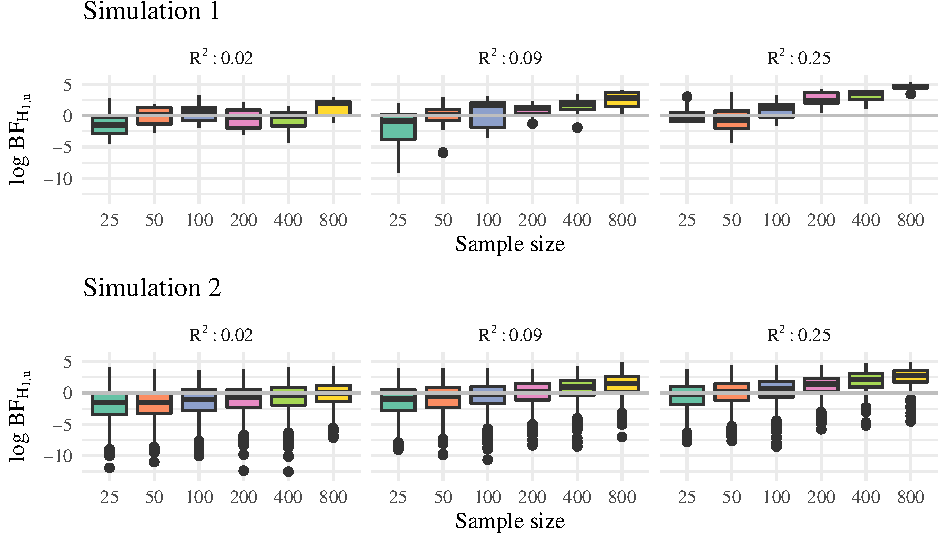
\includegraphics[width=1\linewidth]{manuscript_volker_files/figure-latex/BF12-1} \caption{Aggregated Bayes factors for hypothesis $H_{1,2}: \beta_4 < \beta_5 < \beta_6$ versus $H_u$ over three studies (with linear, logistic and probit models). In simulation 2, one of the three studies is randomly selected to have a small sample size ($n = 25$).}\label{fig:BF12}
\end{figure}

\begin{figure}
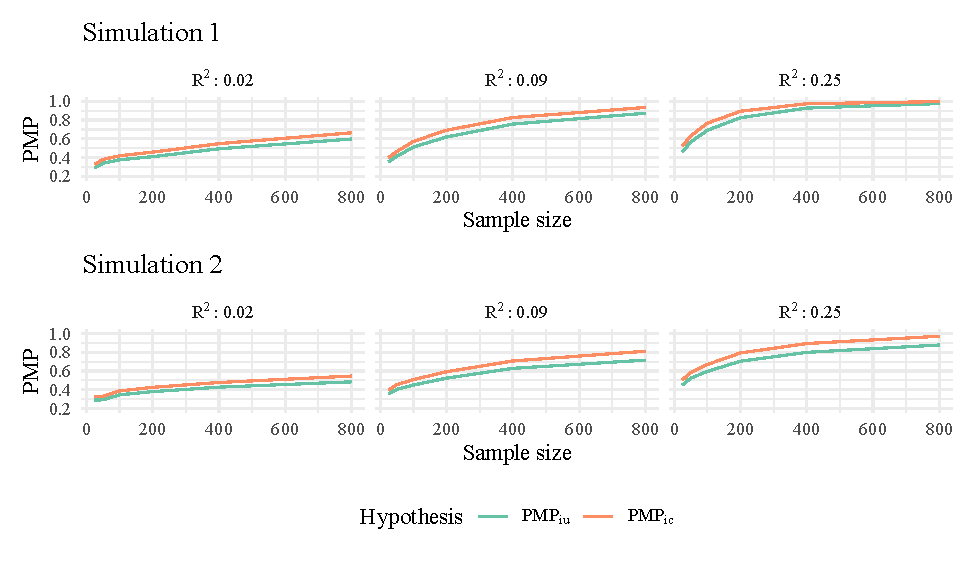
\includegraphics[width=1\linewidth]{manuscript_volker_files/figure-latex/PMP12-1} \caption{Aggregated $PMP$s for hypothesis $H_{1,2}: \beta_4 < \beta_5 < \beta_6$ versus $H_u$ or $H_c$ over three studies (with linear, logistic and probit models). In simulation 2, one of the three studies is randomly selected to have a small sample size ($n = 25$).}\label{fig:PMP12}
\end{figure}

In simulation 1 and 2, the aggregated Bayes factors for the true hypothesis \(H_{1,2}: \beta_4 < \beta_5 < \beta_6\) against the unconstrained hypothesis \(H_u\) increase with sample size and effect size (Figure \ref{fig:BF12}).
In simulation 1, for a small effect size (\(R^2 = 0.02\)), \(H_{1,2}\) is more often supported than \(H_u\) only when the sample size is at least \(n \geq 400\).
For \(n = 400\) and \(R^2 = 0.02\), the median aggregated Bayes factor (the middle horizontal black line in the box) is slightly above zero on the logarithmic scale, indicating that there is more support for the true hypothesis \(H_{1,2}\) than for \(H_u\) in slightly more than \(50\%\) of the iterations.
When the effect sizes increase, \(H_{1,2}\) is preferred over \(H_u\) in most iterations when \(n \geq 100\) or when \(n \geq 50\), for \(R^2 = 0.09\) and \(R^2 = 0.25\), respectively.
Note that when evaluating a hypothesis against an unconstrained alternative, the Bayes factor has an upper bound.
When the hypothesis fits the data perfectly (i.e., \(f_i = 1\)), the Bayes factor within a study cannot exceed \(1/c_i\).
Hence, the aggregated Bayes factor for three studies also has an upper bound.
For \(n = 800\) observations per study and a large effect, the aggregated Bayes factor consistently approaches this upper bound.
In simulation 2, this upper bound is not reached in any condition, as the support for \(H_{1,2}\) is generally smaller than in simulation 1.
Likewise, larger sample sizes and effect sizes are required before \(H_{1,2}\) obtains more support than \(H_u\) in the majority of the iterations.
These findings are to be expected, because studies with the smallest sample size often provide support against \(H_{1,2}\).
Replacing a study with a larger sample size by a study with a sample size of \(n = 25\) thus leads to a decrease in the aggregated support.

Additionally, the aggregated support for the true hypothesis \(H_{1,2}\) versus both the unconstrained and complement hypothesis is quantified as posterior model probabilities (\(PMP\)s; Figure \ref{fig:PMP12}).
These results also show that the support for the true hypothesis increases with the sample and effect size.
For the smallest effect size, the average aggregated support does not exceed \(0.70\), indicating that \(H_{1,2}\) is hardly favored over \(H_u\).
For medium and large effects, the \(PMP\)s tend to \(1\) when the sample size is large enough.
Comparing simulation 1 and 2 shows that considering a single underpowered study in the set of studies substantially reduces the average aggregated \(PMP\)s.
When the effect size equals \(R^2 = 0.09\), the average aggregated support is larger for three studies with a sample size of \(n = 400\) (in simulation 1) than for two studies with a sample size of \(n = 800\) and one study with \(n = 25\) (in simulation 2).
Hence, although the total number of observations is higher in the latter setting, the average support for the true hypothesis is not, regardless of the alternative hypothesis.
Lastly, Figure \ref{fig:PMP12} shows that evaluating against the complement hypothesis consistently renders more support for the true hypothesis, although the difference is relatively small.

\hypertarget{simulation-3-and-4}{%
\subsubsection{Simulation 3 and 4}\label{simulation-3-and-4}}

\begin{figure}
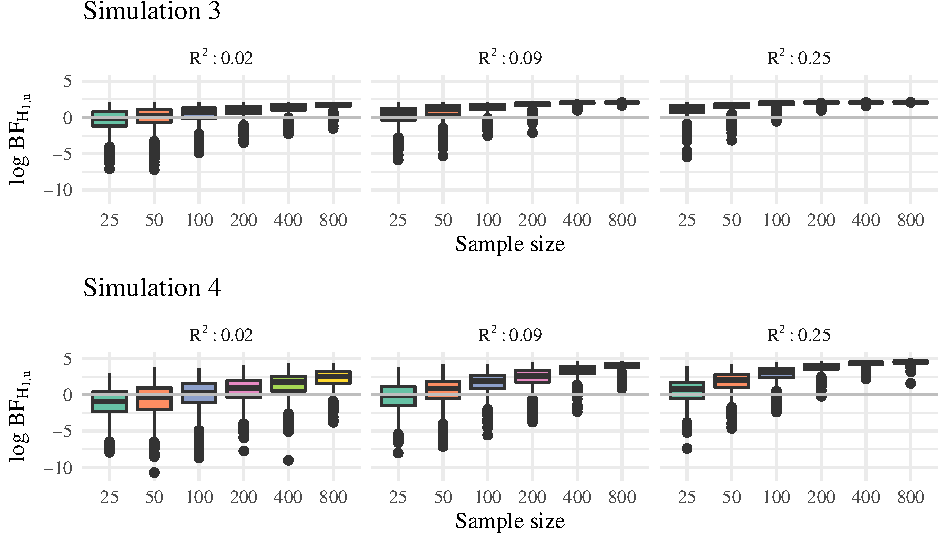
\includegraphics[width=1\linewidth]{manuscript_volker_files/figure-latex/BF34-1} \caption{Aggregated Bayes factors for hypothesis $H_3: \beta_6 > 0$ in simulation 3 and $H_4: \beta_{\text{low}} < \beta_{\text{medium}} < \beta_{\text{high}}$ in simulation 4 versus $H_u$ over three studies (with linear, logistic and probit models).}\label{fig:BF34}
\end{figure}

\begin{figure}
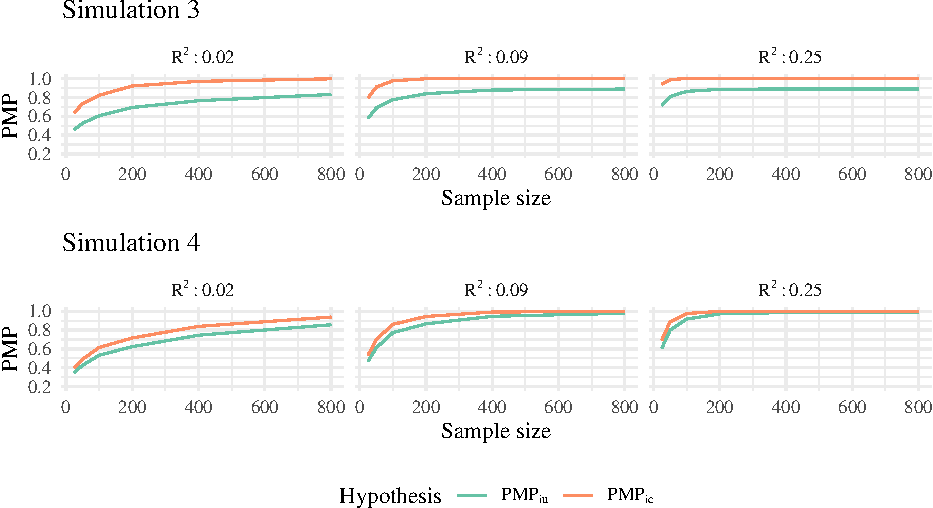
\includegraphics[width=1\linewidth]{manuscript_volker_files/figure-latex/PMP34-1} \caption{Aggregated $PMP$s for hypothesis $H_3: \beta_6 > 0$ in simulation 3, and for $H_4: \beta_{\text{low}} < \beta_{\text{medium}} < \beta_{\text{high}}$ in simulation 4 $H_u$ or $H_c$ over three studies (with linear, logistic and probit models).}\label{fig:PMP34}
\end{figure}

Simulations 3 and 4 assess how the complexities of the hypotheses under consideration affect \emph{BES}, by using different operationalizations of a construct of interest.
In both simulations, we consider the expectation that \(X_6\) and \(Y\) are positively related (after controlling for \(X_1\) to \(X_5\)).
In simulation 3, \(X_6\) is considered as is, such that the hypothesis \(H_3: \beta_6 > 0\) is evaluated.
In simulation 4, \(X_6\) is categorized into equally sized tertiles in each study, corresponding to \emph{low}, \emph{medium} and \emph{high} scoring groups \citep[which is, despite advice against this procedure, common practice in many areas of research; e.g.,][]{bennette_against_2012, decoster_best_2011}.
Capturing the expected positive relationship between \(X_6\) and \(Y\) into an informative hypothesis yields \(H_4: \beta_{\text{low}} < \beta_{\text{medium}} < \beta_{\text{high}}\), where each coefficient reflects the mean of that group controlled for the 5 other variables.
Consequently, the complexity of \(H_4\) is substantially smaller than the complexity of \(H_3\), because more constraints are placed on the parameters.
Note, however, that categorizing a continuous variable also reduces the information in this variable, resulting in less statistical power.

Both Figure \ref{fig:BF34} and Figure \ref{fig:PMP34} show that the support for the true hypotheses \(H_3:\beta_6>0\) and \(H_4: \beta_{\text{low}} < \beta_{\text{medium}} < \beta_{\text{high}}\) increases with sample and effect size.
This is a recurrent pattern when the hypothesis under consideration is in line with the specifications of the parameters.
In simulation 3, \(H_3\) obtains more support than \(H_u\) in more than \(50\%\) of the iterations when the sample size is at least \(n \geq 50\) for small effect sizes.
When medium and large effect sizes are considered, all sample sizes yield more support for \(H_3\) than \(H_u\) in the majority of the iterations.
For all effect sizes, the aggregated Bayes factor tends to its maximum if the sample size is large enough.
The complexity of a one parameter hypothesis with a symmetric prior centered at the boundary of the hypothesis equals \(0.5\).
Hence, aggregating the results of three studies yields a maximum Bayes factor of \((1/0.5)^3\), which is approximately equal to \(2.08\) on a logarithmic scale.
When \(R^2 = 0.02\) in simulation 4, there is, in contrast to simulation 3, initially more support for \(H_u\) than for the hypothesis of interest.
Additionally, the true hypothesis \(H_4\) obtains less support than \(H_3\) in simulation 3 for the smallest sample and effect sizes considered (i.e., for \(n \leq 100\) when \(R^2 = 0.02\), \(n \leq 50\) when \(R^2 = 0.09\) and for \(n = 25\) when \(R^2 = 0.25\)).
Both findings are the result from \(H_4\) having a smaller complexity than \(H_3\), which requires more statistical power to find support.
Yet, categorizing \(X_6\) yields less statistical power.
Whereas the aggregated support for \(H_3\) quickly reaches its maximum, the support for \(H_4\) continues to increase to higher levels.
For \(n = 800\) when \(R^2 = 0.09\), and for \(n \geq 400\) when \(R^2 = 0.25\), the support for \(H_4\) also reaches its maximum, but this maximum is substantially higher than the maximum in simulation 3, because the complexity of the hypothesis is smaller than in simulation 3.

The posterior model probabilities also clearly pinpoint the upper bound of the support for \(H_3\) when evaluated against \(H_u\) (Figure \ref{fig:PMP34}), especially for medium and large effects.
When \(H_3\) obtains full support from the data, the posterior model probabilities cannot exceed \(8/9\).
The support against the complement hypothesis is unrestricted, and therefore the support for \(H_3\) quickly tends to \(1\) for all effect sizes when compared to the complement hypothesis.
In simulation 4, the complexity of hypothesis \(H_4\) is relatively small.
Compared to simulation 3, the aggregated support for the more complex hypothesis \(H_4\) evaluated against \(H_u\) is therefore smaller for small sample sizes, but continues to increase to almost 1 when the support for \(H_3\) reaches its upper bound.
Additionally, there is only a small difference between evaluating \(H_4\) against the unconstrained and the complement hypothesis: the support for \(H_4\) is unconvincing initially, but increases with the sample and effect size for both alternatives.

\hypertarget{simulation-5-and-6}{%
\subsubsection{Simulation 5 and 6}\label{simulation-5-and-6}}

Simulations 5 and 6 also examine how evaluating hypotheses with different complexities affects \emph{BES} by varying the operationalizations of key constructs.
Assume that the variables \(X_2\), \(X_3\) and \(X_4\) are indicators of the same theoretical construct.
In simulation 5, the three indicators are collapsed into a single scale variable \(X_{\text{scale}}\) by taking the average of these variables for each observation in each of the studies, which is common scientific practice \citep{bauer_discrepancy_2016}.
Accordingly, the hypothesis under evaluation is \(H_5: \beta_{\text{scale}} > 0\), analysed in a model including an intercept and \(X_1\), \(X_5\) and \(X_6\) as control variables.
In simulation 6, the variables are left as is and included separately in the analyses, such that hypothesis \(H_6: \{\beta_2,\beta_3,\beta_4\} > 0\) is evaluated (with the same control variables).
Due to these specifications, \(H_5\) has a larger complexity than \(H_6\), due to \(H_6\) addressing multiple parameters, while \(\beta_{\text{scale}}\) has a smaller standard error than each of the individual regression coefficients (\(\beta_2\), \(\beta_3\) or \(\beta_4\)), resulting in more power to detect an effect.

In simulation 5, \(H_5\) obtains more support than \(H_u\) in more than \(50\%\) of the iterations over all sample and effect sizes except for \(n = 25\) and \(R^2 = 0.02\).
Additionally, the aggregated support for \(H_5: \beta_{\text{scale}}>0\) reaches its maximum for medium and large effect sizes (at \(n \geq 400\) and \(n \geq 100\) for \(R^2 = 0.09\) and \(R^2 = 0.25\), respectively).
In simulation 6, where hypothesis \(H_6\) concerns the separate predictors, the pattern is rather different.
When the effect size is small, the unconstrained hypothesis obtains most support, unless the sample size is at least \(n = 400\).
For medium and large effect sizes, \(H_6\) obtains more support than \(H_u\) when \(n \geq 100\) and \(n \geq 50\), respectively, and the support tends to much higher levels than in simulation 5.

Figure \ref{fig:PMP56} for simulation 5 and 6 shows a similar pattern as Figure \ref{fig:PMP34} for simulation 3 and 4.
The support for \(H_5\) when compared with \(H_u\) tends to its maximum, especially for a large effect, while comparing against the complement leads to \(PMP\)s close to \(1\) (at \(n = 800\), \(n \geq 200\) and \(n \geq 50\) for small, medium and large effects, respectively).
In simulation 6, evaluating \(H_6\) against \(H_u\) yields a considerably higher maximum \(PMP\) than in simulation 5, due to the rather small complexity of \(H_6\).
Accordingly, there is almost no difference between evaluating \(H_6\) against \(H_u\) or \(H_c\).
For small effect sizes, \(H_6\) is barely supported for all sample sizes.
Only when both the sample and effect size are sufficiently large, \(H_6\) obtains convincing support.
Hence, when evaluating against an unconstrained alternative, the support for the more specific hypothesis \(H_6\) increases to higher levels than the support for \(H_5\).
These results show the importance of having adequately powered studies when evaluating a specific hypothesis, because only then this hypothesis obtains convincing support.

\begin{figure}
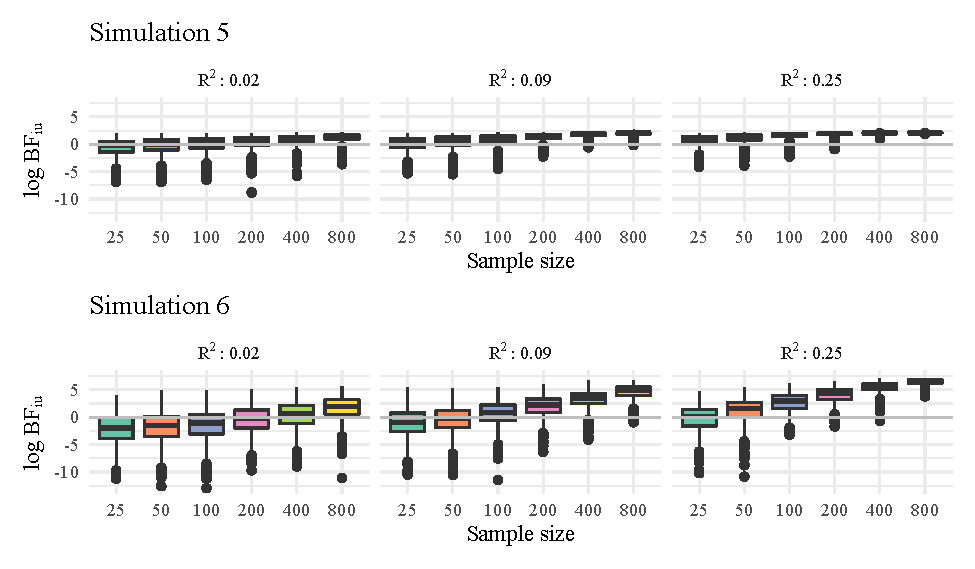
\includegraphics[width=1\linewidth]{manuscript_volker_files/figure-latex/BF56-1} \caption{Aggregated Bayes factors for hypothesis $H_5: \beta_{\text{scale}} > 0$ versus $H_u$ in simulation 5 and $H_6: \{\beta_2, \beta_3, \beta_4\} > 0$ in simulation 6 versus $H_u$ over three studies (with linear, logistic and probit models).}\label{fig:BF56}
\end{figure}

\begin{figure}
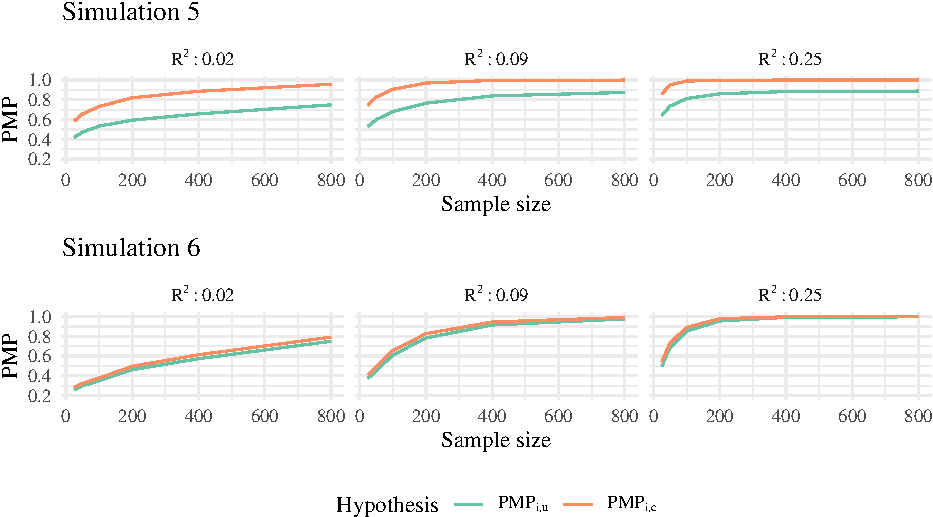
\includegraphics[width=1\linewidth]{manuscript_volker_files/figure-latex/PMP56-1} \caption{Aggregated $PMP$s for hypothesis $H_5: \beta_{\text{scale}} > 0$ in simulation 5 and $H_6: \{\beta_2, \beta_3, \beta_4\} > 0$ in simulation 6 versus $H_u$ or $H_c$ over three studies (with linear, logistic and probit models).}\label{fig:PMP56}
\end{figure}

\hypertarget{simulation-7-and-8}{%
\subsubsection{Simulation 7 and 8}\label{simulation-7-and-8}}

\begin{figure}
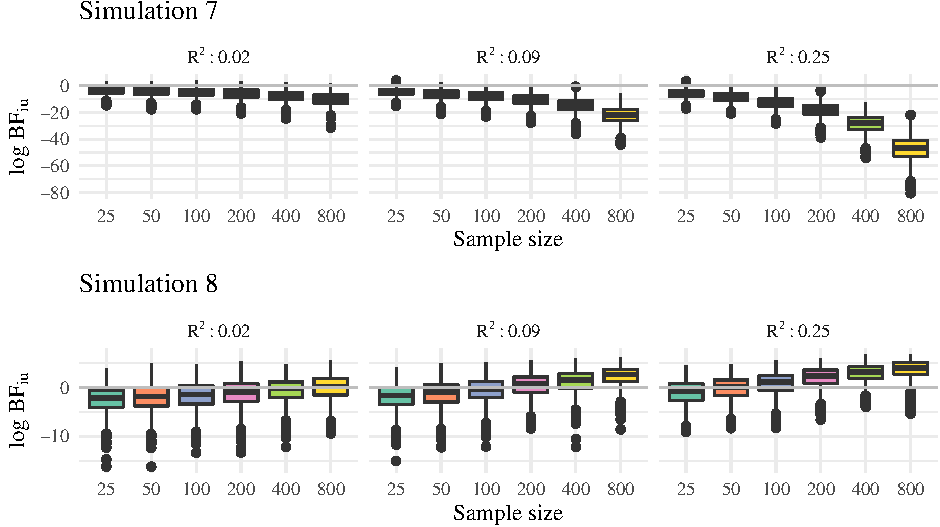
\includegraphics[width=1\linewidth]{manuscript_volker_files/figure-latex/BF78-1} \caption{Aggregated Bayes factors for the \textit{incorrect} hypothesis $H_7: \{\beta_2, \beta_3, \beta_4\} < 0$ in simulation 7 and \textit{partially incorrect} hypothesis $H_8: \{\beta_1, \beta_2, \beta_3\} > 0$ in simulation 8 versus $H_u$ over three studies (with linear, logistic and probit models). Note the different scaling of the y-axis.}\label{fig:BF78}
\end{figure}

\begin{figure}
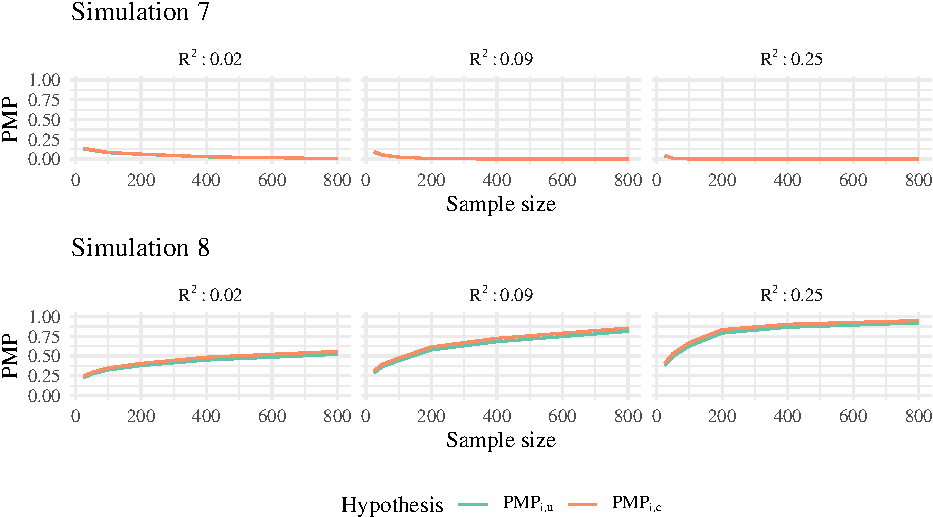
\includegraphics[width=1\linewidth]{manuscript_volker_files/figure-latex/PMP78-1} \caption{Aggregated $PMP$s for the \textit{incorrect} hypotheses $H_7: \{\beta_2, \beta_3, \beta_4\} < 0$ in simulation 7 and $H_8: \{\beta_1, \beta_2, \beta_3\} > 0$ in simulation 8 versus $H_u$ or $H_c$ over three studies (with linear, logistic and probit models).}\label{fig:PMP78}
\end{figure}

All previous simulations were concerned about whether \emph{BES} provides adequate results when a correct informative hypothesis is evaluated against the unconstrained or complement hypotheses.
In simulation 7 and 8, we assess the performance of \emph{BES} when the hypothesis of interest is incorrect.
We therefore expect \emph{BES} to render \emph{less} support for the hypotheses of interest when the sample and effect size increase.
In simulation 7, we consider \(H_7: \{\beta_2, \beta_3, \beta_4\} < 0\), implying a negative relationship between the indicators \(X_2\), \(X_3\) and \(X_4\) and the outcome \(Y\), which is in the opposite direction as hypothesis \(H_6\) evaluated in simulation 6.
Hence, the unconstrained and complement alternative hypotheses are correct, although rather unspecific, in these simulations.
In simulation 8, we evaluate \(H_8: \{\beta_1, \beta_2, \beta_3\} > 0\), which is correct for \(\beta_2\) and \(\beta_3\), but incorrect for \(\beta_1\), because \(\beta_1 = 0\).
Hypothesis \(H_8\) is a challenging hypothesis to evaluate, because the sampling distribution of \(\beta_1\) is symmetrically centered around 0, which is on the boundary of the hypothesis of interest.
The posterior mean of \(\beta_1\) will therefore be in line with \(H_8\) in about \(50\%\) of the iterations.
Accordingly, the unconstrained hypothesis is correct in these simulations, while the complement hypothesis is also partially incorrect, because the true parameter value is exactly on the boundary of \(H_8\) and \(H_c\).

Figure \ref{fig:BF78} shows the support for the \emph{incorrect} hypothesis \(H_7: \{\beta_2, \beta_3, \beta_4\} < 0\) and \emph{partially incorrect} hypothesis \(H_8: \{\beta_1, \beta_2, \beta_3\} > 0\).
In simulation 7, the support for the incorrect hypothesis of interest quickly decreases, and renders more support for the unconstrained hypothesis.
In fact, already from the smallest sample sizes onward, there is more support for the \emph{correct} unconstrained hypothesis than for \(H_7\), which is amplified when the sample and effect size increase.
In simulation 8, the support for the partially incorrect hypothesis \(H_8\) increases, rather than decreases, with the sample size and effect size (Figure \ref{fig:BF78}; note the different scale of the y-axis compared to simulation 7).
Whereas for small sample and effect sizes the \emph{correct} unconstrained hypothesis is preferred over \(H_8\), the \emph{incorrect} hypothesis \(H_8\) eventually obtains more support.
Although this behavior is undesirable, it is not surprising.
For larger sample and effect sizes, the posterior distribution of two of the three regression coefficients will be completely in line with the constraints imposed by \(H_8\), whereas the posterior of \(\beta_1\) is, on average, also for \(50\%\) in line with this hypothesis.
Hence, even though the hypothesis is partially incorrect, the fit generally exceeds the complexity.

The posterior model probabilities tell a similar story (Figure \ref{fig:PMP78}).
The average aggregated \(PMP\)s for the incorrect \(H_7\) render very strong support against this hypothesis, for all sample sizes and effect sizes and for both alternative hypotheses (the lines for \(H_u\) and \(H_c\) are almost completely overlapping).
In simulation 8, the average aggregated \(PMP\)s are indecisive under a small effect size, but favor the partially incorrect hypothesis \(H_8\) over the correct unconstrained and partially incorrect complement hypothesis when the effect and sample size increase.
The difference between evaluating against \(H_u\) and \(H_c\) is negligible, although \(H_u\) is the only correct hypothesis in this simulation, because \(\beta_1\) is also on the boundary of the admissible parameter space of \(H_c\).

In both simulations 7 and 8, the unconstrained hypothesis is preferred over the (partially) incorrect hypotheses for the smallest sample and effect sizes.
Although this is, of course, desirable behavior, it may sketch an overly optimistic picture.
Namely, in simulation 6, we evaluated a similar hypothesis in terms of complexity (i.e., \(H_6: \{\beta_2, \beta_3, \beta_4\} > 0\)).
This simulation also rendered more support for the unconstrained hypothesis.
Hence, these results predominantly show that when the estimates are noisy due to little statistical power, less specific hypotheses obtain more support than more specific hypotheses.

\hypertarget{discussion-simulations-part-1}{%
\subsubsection{Discussion simulations part 1}\label{discussion-simulations-part-1}}

Part one of the simulations provides insight in the performance of \emph{BES}, when studies consider conceptually similar hypotheses with different complexities due to different operationalizations.
Simultaneously, part one demonstrated the importance of the statistical power in the individual studies.
Our simulations show that \emph{BES} performs adequately when the individual studies have sufficient statistical power given the complexity of the hypothesis.
The support for specific, correct hypotheses consistently increase with the sample and effect size.
Hence, \emph{BES} allows to evaluate rather precise hypotheses, constraining multiple parameters, as long as the sample size and effect size are large enough.
Also if the hypothesis of interest is incorrect, as in simulation 7, the correct unconstrained hypothesis obtains considerable support.
Yet, a hypothesis that is correct on multiple parameters and not too far from correct on the remaining parameters can obtain considerable support, as shown in simulation 8.
If a substantial region of the joint posterior is in line with the hypothesis, as in these simulations, the fit of the hypothesis may still exceed the complexity.
Note, however, that although the aggregated support for the hypothesis may be considerable, the results within the individual studies are likely to raise doubts.
That is, even though the overall hypothesis may be supported, the estimated parameters fluctuate around their true values.
If the estimated coefficients in the individual studies are often not in line with the hypothesis, this is an indication that further there might be something else going on, even though the overall hypothesis obtains substantial support.
Hence, the results in the individual studies may still suggest that the theory can be improved and the hypotheses can be refined and evaluated, albeit with new data.

The results also show that the specification of the alternative hypothesis has consequences for \emph{BES}.
Evaluating against a complement alternative hypothesis yields a more powerful evaluation of the hypothesis than evaluating against the unconstrained hypothesis.
Additionally, when the hypothesis of interest has a relatively large complexity and the studies have sufficient statistical power, the aggregated support quickly tends to its upper bound when evaluating against an unconstrained hypothesis.
Comparing against the complement hypothesis yields no upper bound for the aggregated support, and the aggregated evidence reflects the amount of evidence that is obtained within each study more accurately.
When the complexity of the hypothesis of interest is sufficiently small, the upper bound of the aggregated support increases, such that the difference between evaluating against the unconstrained or complement hypothesis becomes negligible in terms of posterior model probabilities.

Lastly, we find that having sufficient statistical power in the individual studies is an important requirement.
The inclusion of underpowered studies therefore decreases the performance of \emph{BES}, as shown in simulation 1 and 2.
As the results show, including three adequately powered studies provides more convincing support for the true hypothesis than the inclusion of two adequately powered studies and a single underpowered study, even if the total number of observations in the latter scenario is larger.
The need for adequately powered studies increases when evaluating very specific hypotheses (i.e., hypotheses with a small complexity, imposing multiple constraints on the parameters).
That is, if the parameters cannot be estimated very accurately due to noisy data or a small sample, it becomes likely that at least one of the constraints imposed by the hypothesis are violated.
Common procedures in data handling, such as categorizing continuous variables, which simultaneously reduce the complexity of the hypothesis and the statistical power, may therefore have adverse consequences for \emph{BES}.
Likewise, evaluating hypotheses that simultaneously assess multiple indicators requires more statistical power than evaluating a hypothesis on a single parameter, as a factor score.
For the smallest sample sizes and effect sizes, evaluating such specific hypotheses renders more support for the unconstrained and complement hypotheses than for the hypothesis of interest.
This implies that adding more studies that all lack statistical power results in less, rather than more support for the true hypothesis.
Altogether, these results emphasize that \emph{BES} is not a data pooling technique, but rather quantifies the extent to which a hypothesis is supported over multiple studies.
We further address the consequences of this issue in the subsequent section.

\hypertarget{simulations-part-2---small-sample-issues}{%
\subsection{Simulations part 2 - small sample issues}\label{simulations-part-2---small-sample-issues}}

The previous section underscores that there remains considerable uncertainty about the sensitivity of \emph{BES} to the sample size and effect size of the individual studies.
Part two of the simulations zooms in on the extent to which \emph{BES} renders support for \emph{correct} hypotheses as the number of studies increases.
Moreover, we assess the influence of the choice of alternative hypothesis (i.e., an unconstrained or a complement alternative hypothesis) on the amount of aggregated support.
In the second set of simulations, we consider the same data-generating mechanism as in previous simulations, but restrict the simulations to OLS regression (using other models yields equivalent results).\footnote{
  In this situation, approaches like meta-analysis and Bayesian sequential updating would be feasible. A comparison of methods is, however, beyond the scope of this paper.}
Hence, in all simulations, the outcome \(Y\) is generated from a normal distribution (i.e., \(Y \sim \mathcal{N}(X\beta, 1 - R^2)\)), and analysed using OLS regression model including an intercept and all predictors \(X\).
To keep the results tractable, only one effect size and two sample sizes are considered (\(R^2 = 0.09\) and \(n \in \{25, 200\}\)), representing an underpowered and an adequately powered study.
In contrast to the previous simulations, the number of studies is varied from \(1\) to \(150\).
In all four simulations in part two, the cumulative aggregated support is assessed for the hypotheses of interest against an unconstrained and a complement alternative hypothesis for the two sample sizes considered.

\hypertarget{simulations-9-and-10}{%
\subsubsection{Simulations 9 and 10}\label{simulations-9-and-10}}

\begin{figure}[t]
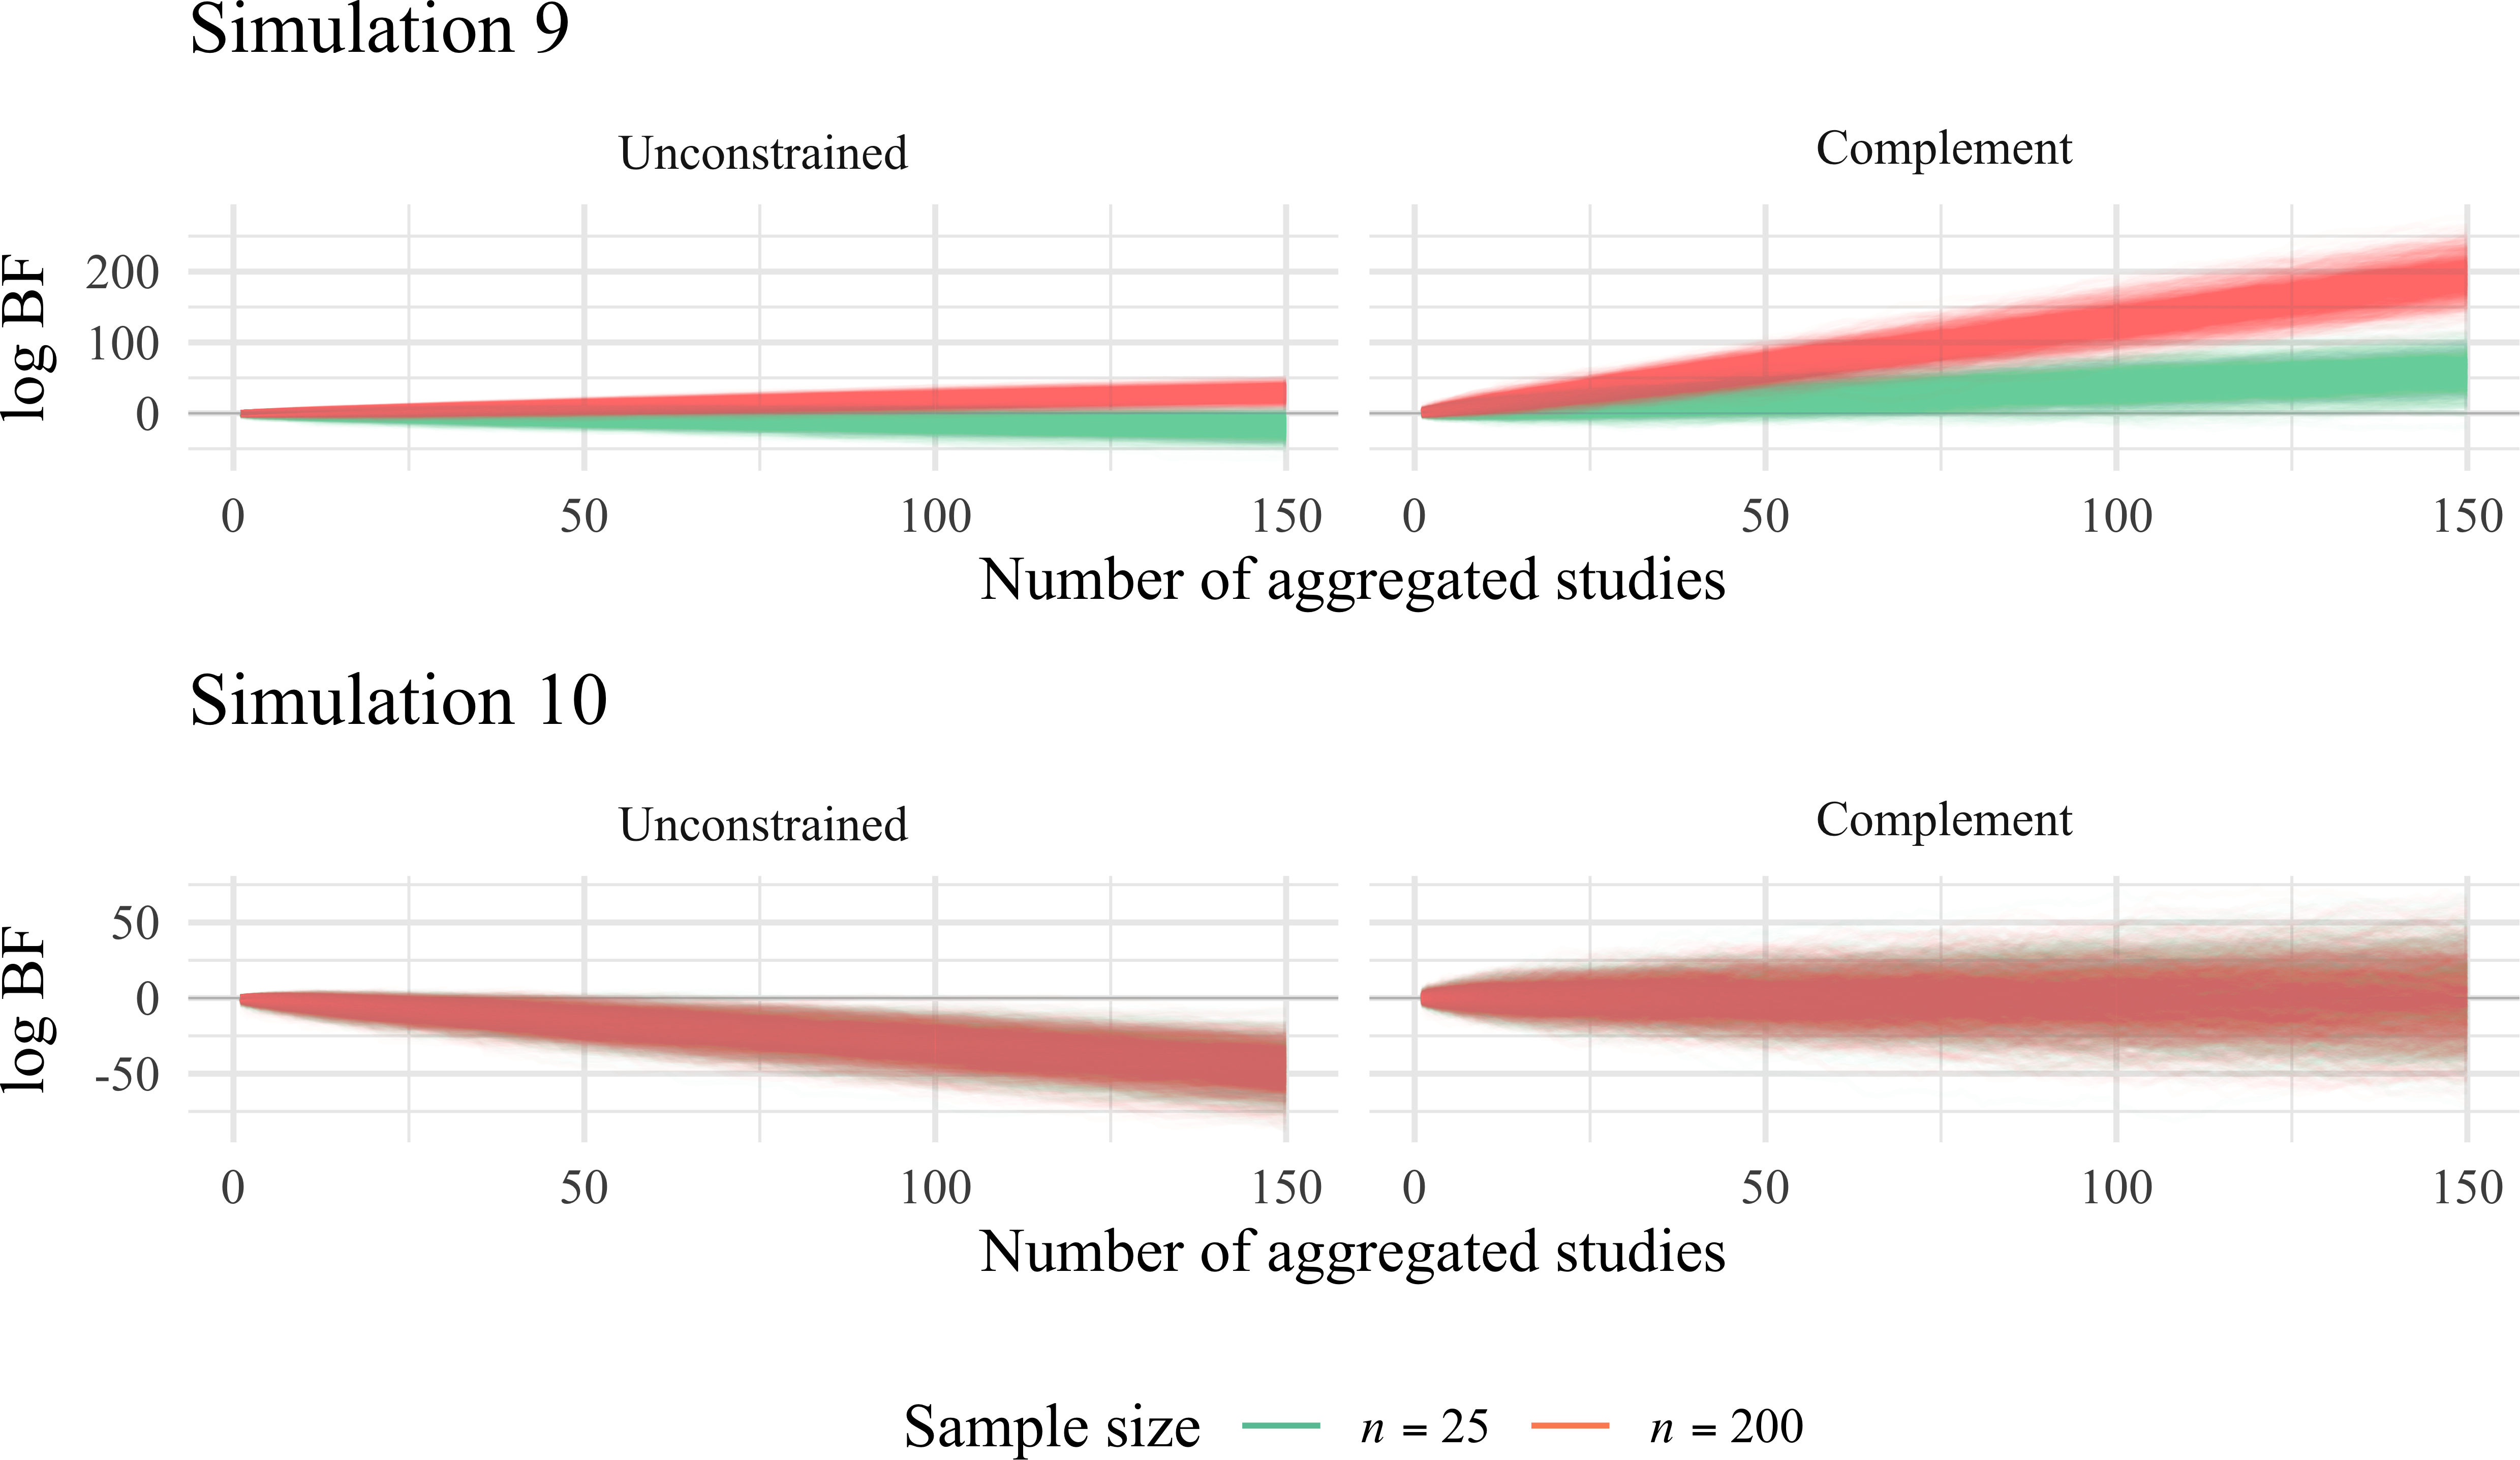
\includegraphics[width=1\linewidth]{manuscript_volker_files/figure-latex/simBF910-1} \caption{Cumulative aggregated Bayes factors for the correct hypothesis $H_9: \beta_2 > 0$ in simulation 9 and $H_{10}: \beta_1 > 0$ in simulation 10, versus an unconstrained and complement alternative hypothesis over 1 to 150 studies, based on an OLS regression model. Note (i) that the scale of the y axis differs between the two simulations, and (ii) that the lines for the two sample sizes are completely overlapping in simulation 10.}\label{fig:simBF910}
\end{figure}

In simulation 9, we evaluate hypothesis \(H_9: \beta_2 > 0\) against the unconstrained and complement hypotheses and assess the influence of the alternative hypothesis for underpowered and adequately powered studies.
Recall that \(H_9\) is correct, as the population value of the coefficient equals \(\beta_2 = 0.054\) (Table \ref{tab:coefs}).
Figure \ref{fig:simBF910} shows that, for studies with a small sample size (i.e., \(n = 25\); the green lines in Figure \ref{fig:simBF910}), evaluating against \(H_u\) yields decreasing support for the correct hypothesis \(H_9\) when the number of studies considered increases.
That is, for small sample sizes, \(H_u\) is clearly preferred over \(H_9\), and although the former is correct, it is not informative at all.
For larger samples (i.e., \(n = 200\)), the correct hypothesis \(H_9\) is preferred over \(H_u\).
Yet, the aggregated support increases at a rather slow rate, due to the fact that the aggregated support has an upper bound.
Evaluating \(H_9\) against the \emph{incorrect} complement hypothesis consistently renders support for the former, regardless of the sample size.
Additionally, the support for \(H_9\) when evaluated against \(H_u\) increases at a faster rate than when evaluated against \(H_c\), due to the absence of an upper bound.

Yet, there is a downside to evaluating against the complement hypothesis, that becomes apparent when evaluating a hypothesis that is constrained at the true parameter value.
In simulation 10, we evaluate the hypothesis \(H_{10}: \beta_1 > 0\) while the true parameter value equals \(\beta_1 = 0\).
If the true effect of the parameter is on the boundary of the hypothesis of interest and its complement, there is substantial variability in the support, regardless of the sample size (note that the lines for the two sample sizes are completely overlapping for simulation 10).
Specifically, although \(H_{10}\) and \(H_c\) obtain, on average, the same support over all iterations, the individual iterations show considerable support for either of the two.
A researcher can thus find considerable support for or against an hypothesis on the aggregate level, while there is no effect in reality.
When evaluating against the unconstrained hypothesis, the support for the incorrect hypothesis \(H_{10}\) decreases as more studies are added, regardless of the sample size (note again that the lines for the two sample sizes are completely overlapping).

\hypertarget{simulations-11-and-12}{%
\subsubsection{Simulations 11 and 12}\label{simulations-11-and-12}}

The previous two simulations assessed the difference between evaluating a hypothesis on one parameter against an unconstrained and complement alternative.
If the prior distribution of the parameter is centered around the constraint imposed by the hypothesis, this results in the fact that the hypothesis of interest and its complement are balanced, in the sense that both hypotheses have a complexity of \(1/2\).
In simulation 11, a hypothesis with constraints on multiple parameters \(H_{11}: \{\beta_2, \beta_3, \beta_4\} > 0\), which is the same hypothesis as evaluated in simulation 6, is evaluated against an unconstrained and complement alternative.
Hypothesis \(H_{11}\) is a correct hypothesis (i.e., \(\beta_2 = \beta_3 = \beta_4 = 0.054\); Table \ref{tab:coefs}), but it is not balanced with its complement, because \(H_{11}\) has a smaller complexity.

Simulation 11 in Figure \ref{fig:simBF11} shows that the support for the correct hypothesis \(H_{11}\) decreases when more small sample studies are included, regardless of the alternative hypothesis.
Hence, when the complexity of the hypothesis of interest and its complement are not balanced, the aggregated Bayes factor does not necessarily tend to the \emph{correct} hypothesis, but favors the more general hypothesis.
When the sample size is sufficiently large, the issue dissolves, and the support for \(H_{11}\) increases substantially when more studies are added.
This finding complements the results from part one of the simulations, in the sense that evaluating fairly specific hypothesis is only feasible when there is sufficient statistical power.
Otherwise, more general hypotheses tend to be preferred over more specific hypotheses.

\begin{figure}[!t]
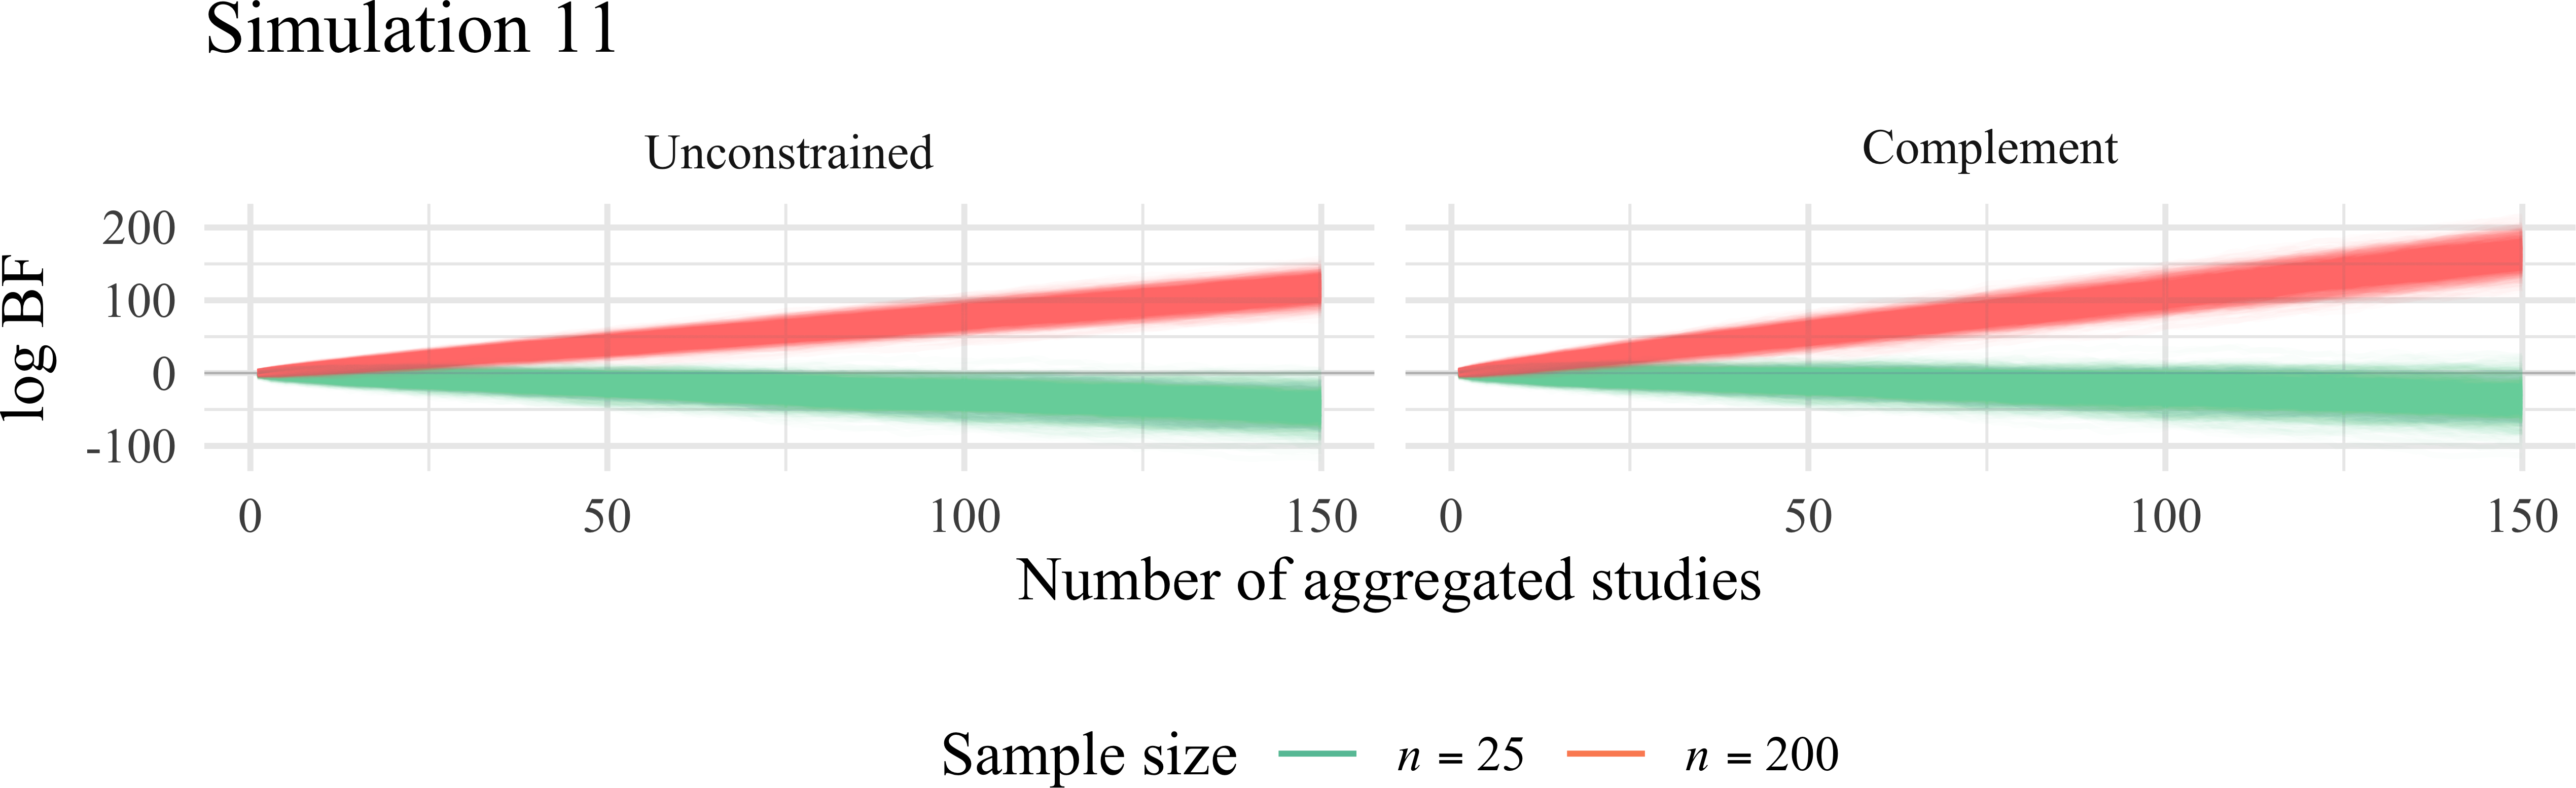
\includegraphics[width=1\linewidth]{manuscript_volker_files/figure-latex/simBF11-1} \caption{Cumulative aggregated Bayes factors for hypothesis $H_{11}: \{\beta_2, \beta_3, \beta_4\} > 0$ in simulation 11 versus $H_u$ and $H_c$ over 1 to 150 studies. In simulation 12, the hypothesis space is separated in three parts ($H_{12_a}: \beta_2 > 0$, $H_{12_b}: \beta_3 > 0$ and  $H_{12_c}: \beta_4 > 0$), evaluated against their respective complements and an unconstrained hypothesis.}\label{fig:simBF11}
\end{figure}

If researchers still want to aggregate support for hypotheses on multiple parameters, even though the individual studies likely lack statistical power, it is possible to simplify the hypothesis of interest.
Complex informative hypotheses on multiple parameters can often be separated in multiple, simpler hypotheses.
In simulation 12, the hypothesis \(H_{11}\) is deconstructed into three simpler hypotheses (\(H_{12_a}: \beta_2 > 0\), \(H_{12_b}: \beta_3 > 0\) and \(H_{12_c}: \beta_4 > 0\)).
Each hypothesis is evaluated against the unconstrained hypothesis, and against its complement.
Note that this procedure yields that each hypothesis is balanced with its complement.
Using this set-up, all hypotheses obtain considerable support when compared to their respective complements for both sample sizes.
Hence, whereas evaluating a complex hypothesis as \(H_{11}\) in simulation 11 leads to support against the hypothesis of interest, evaluating the separate components of the hypothesis in simulation 12 provides support for each component.
Evaluating each components against the unconstrained hypothesis results in support for \(H_u\) when the sample size is small, whether the separate components obtain more support when the sample size is large enough (which is similar to simulation 9 in Figure \ref{fig:simBF910}).

\hypertarget{discussion-simulation-part-2}{%
\subsubsection{Discussion simulation part 2}\label{discussion-simulation-part-2}}

Part two of the simulations focused on the applicability of \emph{BES} when the individual studies lack statistical power.
Aggregating support over studies with relatively few observations, arguably unreasonably few for a regression model with \(6\) predictors, always yields more support for the unconstrained hypothesis than for a correct, and more specific, hypothesis.
If the individual studies lack statistical power, the parameter estimates in these studies vary considerably.
Accordingly, the estimated parameters will occasionally contradict the hypothesis of interest, providing evidence against this hypothesis.
Evaluating against an unconstrained hypothesis yields that evidence against the hypothesis of interest weighs heavier than evidence for this hypothesis.
That is, when evaluating a hypothesis against the unconstrained, the Bayes factor within each study has an upper bound, but no lower bound.
Consider that one study finds, by chance, substantial support against the hypothesis of interest (e.g., with complexity \(c_i = 0.5\) and fit \(f_i = 0.1\), such that \(BF_{i,u} = 0.2\)).
Incorporating two additional studies that perfectly fit the hypothesis of interest still yields more support for the unconstrained hypothesis than for the hypothesis of interest.
Evaluating against a complement alternative weighs evidence for and against the hypothesis of interest equally heavy.
If the hypothesis of interest has a complexity of \(0.5\), the aggregated support will eventually favor the true hypothesis, if either the hypothesis of interest or its complement is correct.

When the hypothesis of interest places constraints on multiple parameters, resulting in a specific hypothesis with a small complexity, evaluating against its complement is not guaranteed to converge toward support for the \emph{correct} hypothesis.
Consider the hypothesis \(H_i: \{\beta_1, \beta_2, \beta_3\} > 0\), which reflects one ordering out of eight possible orderings of the parameters (i.e., each parameter is greater than 0 or it is not, resulting in \(2^3\) possible orderings).
Accordingly, the hypothesis \(H_i\) can be wrong in multiple but one ways.
In studies with insufficient power, estimates vary considerably around the true parameter values, increasing the likelihood that at least one of the constraints imposed by the hypothesis is violated.
Accordingly, in every study a different constraint can be violated, resulting in a relatively poor fit of the hypothesis in each of the studies, such that the aggregated evidence contradicts the hypothesis.
This deficiency can be remedied by dividing the hypothesis space in smaller regions, and evaluating each part separately against its complement.
If each sub-hypothesis and its complement are balanced, the aggregated evidence will support the correct hypothesis.
Hence, this approach allows to assess whether each component of the hypothesis obtains support after aggregation.
Moreover, if the overall hypothesis is incorrect, evaluating the sub-hypotheses highlights which aspects of the overall hypothesis are not supported.
Evaluating the sub-hypotheses is therefore valuable to further refine the theory, after which new data can be collected and the refined hypothesis can be evaluated.

Yet, although considering sub-hypotheses has certain advantages, it should be used with caution.
Simulation 10 shows that evaluating the support for a hypothesis versus its complements can yield substantial support for either of the two, even if both are incorrect.
This finding has implications beyond \emph{BES}, as it affects hypothesis evaluation using Bayes factors in general.
When the true parameter value is on the boundary of a hypothesis and its complement, it is possible to find seemingly overwhelming support for one of the two, while the supported hypothesis is incorrect.
When more studies are included, the variability of the aggregated support increases and the problem is amplified, in the sense that it is rather common to find overwhelming support for one of the two hypotheses.
In such instances, researchers might evaluate the hypothesis of interest against both the unconstrained and the complement hypothesis.
If both render support for (or against) the hypothesis of interest, one can conclude that this hypothesis provides an accurate description to the data.
If the results are contradictory, researchers must acknowledge that considerable uncertainty remains, and that more (adequately powered) studies on the topic are required to make robust scientific claims.

\hypertarget{conclusion}{%
\section{Conclusion}\label{conclusion}}

In multiple simulations, we assessed the ability of Bayesian Evidence Synthesis to evaluate hypotheses with different complexities under various sample and effect sizes.
The first set of simulations showed that \emph{BES} is applicable regardless of differences in analysis models in the set of studies under consideration, and renders correct results if the statistical power on the level of the individual studies is sufficient.
The simulations emphasized the importance of statistical power when aggregating evidence over studies, especially when evaluating specific hypotheses.
When the sample and effect sizes were small, evaluating a hypothesis with a relatively small complexity generally provides more support for the unconstrained and complement hypotheses than for the hypothesis of interest.
If the aggregated Bayes factors within the studies yield more support for the alternatives than for the specific correct hypothesis, adding more studies that are also underpowered will not solve the issue.
In this sense, \emph{BES} clearly differs from conventional methods for research synthesis (e.g., (Bayesian) meta-analysis and Bayesian sequential updating).
Whereas the former two approaches increase the statistical power when incorporating evidence from additional studies, \emph{BES} does not.

Part two of the simulations underscored that adding more underpowered studies only amplifies the issue, to such an extent that aggregating the evidence for hypotheses with a small complexity is unfeasible when the studies lack power, regardless of whether the hypothesis is evaluated against an unconstrained or complement alternative.
If the hypothesis of interest and its complement are balanced, however, the aggregated Bayes factor will eventually show support for the correct hypothesis, if either the hypothesis of interest or its complement is correct.
As a consequence, it can be worthwhile to separate a specific hypothesis with multiple parameter constraints into multiple sub-hypotheses that are all balanced with their complements.
If either the sub-hypothesis or its complement is correct, the aggregated Bayes factor will provide support for the correct hypothesis.
Moreover, evaluating sub-hypotheses allows to assess which constraints imposed by the overall hypothesis are supported by the data and which are not, providing a more detailed overview of the support in the studies for the overall hypothesis.

Evaluating against the complement might, however, be problematic if the true parameter value is on the boundary of the hypothesis of interest and its complement.
In such circumstances, the aggregated support becomes highly variable, and considerable support for either the hypothesis of interest or its complement can be found.
It the studies show that the parameter estimates vary predominantly around the boundary of the hypothesis, a researcher might consider to evaluate an equality-constrained hypothesis, which allows to quantify the plausibility of the absence of an effect.
Yet, evaluating equality-constrained hypotheses with Bayes factors is sensitive to the scale (i.e., variance) of the prior distribution in each study \citep{hoijtink_prior_2021, tendeiro_kiers_2019}.
Accordingly, a sensitivity analysis of the Bayes factor is generally required \citep{hoijtink_prior_2021}, which results in considerable uncertainty with regard to the ``right'' Bayes factor within a study, let alone when aggregated over studies.
This problem is non-existent when evaluating inequality-constrained hypotheses, because in such circumstances, the Bayes factor is insensitive to the prior variance.
Additionally, Bayes factors on equality-constrained hypotheses versus unconstrained alternatives tend to provide overly strong evidence in favor of the former, especially when the power of the study is relatively small \citep[e.g.,][]{tendeiro_kiers_2019}.
The sensitivity of \emph{BES} to power issues might thus become more pronounced when evaluating equality-constrained hypotheses, although future research should address this issue in further detail.
Rather than reverting to point hypotheses, researchers might consider to express the support for a hypothesis of interest against both an unconstrained hypothesis and a complement alternative hypothesis, as the former renders a more conservative way of evaluating informative hypotheses \citep[in line with previous findings by][although this study evaluated hypotheses using an information criterion rather than with Bayes factors]{vanbrabant_complement_2020}.
If the results are robust across alternative hypotheses, researchers can be confident that the hypothesis of interest provides an accurate description of the data.
If the results are not robust, the set of studies might not permit to make strong claims, and more research will be necessary.

Lastly, \emph{BES} has strengths that the conventional methods for research synthesis lack, in the sense that \emph{BES} is capably of dealing with studies that use different designs (i.e., experimental, cross-sectional or longitudinal), have different hierarchical structures, or use different operationalizations of key variables.
Whereas we focused on equivalent operationalizations of key constructs within a set of studies, \emph{BES} allows to aggregate over studies with different operationalizations of important variables.
This may, however, have important implications that future methodological research should address.
When assessing hypotheses with different complexities within the same set of studies, the contribution of each study may depend on the specification of the hypothesis, which in turn affects the aggregated results.
For example, if one of the studies tests a complex hypothesis with multiple constraints, while it does not have the statistical power to evaluate such a hypothesis, the results of this individual study may severely impact the conclusions after aggregation.
Accordingly, researchers should not trust blindly on the results after aggregation, but assess the results in the individual studies as well.
The results on the level of the individual studies may give an additional sense of the robustness of the results over different situations, while simultaneously signifying potential moderating circumstances of the effect of interest.
Such additional information might raise doubts about the robustness of the conclusions in specific scenarios, but can also hint towards interesting new areas of research or corroborate the conclusions from the synthesis.
In sum, \emph{BES} can be used to aggregate scientific evidence over heterogeneous studies.
Yet, solely relying on this aggregate derogates from the wealth of information that can be extracted from the individual studies.

\bibliography{thesis.bib}


\end{document}
